\documentclass[b5paper]{article}
\usepackage{kotex}
\usepackage{amsmath}
\usepackage{amssymb}
\usepackage{titlesec}
\usepackage{graphicx}
\usepackage{units}
\usepackage[utf8]{inputenc}
\usepackage[symbol,perpage]{footmisc}
\usepackage[]{geometry} % 페이지 크기 및 여백 지정
\geometry{verbose, tmargin=2.5cm, bmargin=2.5cm, voffset=0cm, lmargin=1.8cm, rmargin=1.8cm, headheight=4cm, headsep=0.3cm}
%opening
\title{일반상대성 이론의 기초\footnote{- Alfred Engel의 영역본 A. Einstein, \emph{The Foundation of the General Theory of Relativity}, Writings, 1914-1917 - The Collected Papers of Albert Einstein, pp.146-200 을 저본으로 하고, 독일어 원문 A. Einstein, \emph{Die Grundlage der allgemeinen Relativitätstheorie}. Leipzig 1916. 64 S., Abb. (aus: Annalen der Physik. 49 (1916))을 참고함.}}
\date{}
\author{\normalsize A. 아인슈타인(1916) / 편역: 류명선}
\titleformat{\chapter}[hang]{\Large\bfseries}{\thechapter\hsp\textcolor{gray75}{|}\hsp}{0pt}{\Large\bfseries}
\titleformat{\section}[hang]{\large\bfseries}{\thesection\hsp\textcolor{gray75}{|}\hsp}{0pt}{\large\bfseries}
\newcommand\numberthis{\addtocounter{equation}{1}\tag{\theequation}}
\usepackage{parskip}
\usepackage{verbatim}
\setlength{\parindent}{1em}
\setlength{\parskip}{0ex}
\renewcommand{\baselinestretch}{1.3}
\begin{document}

\newcommand{\pderiv}[2]{{\frac{{\partial}{#1}}{{\partial}{#2}}}}
\newcommand{\ppderiv}[3]{{\frac{{\partial^2}{#1}}{{\partial}{#2}{\partial}{#3}}}}
\newcommand{\ilpderiv}[2]{{{{\partial}{#1}}/{{\partial}{#2}}}}
\newcommand{\ilppderiv}[3]{{\frac{{\partial^2}{#1}}/{{\partial}{#2}{\partial}{#3}}}}
\newcommand{\pppderiv}[4]{{\frac{{\partial^3}{#1}}{{\partial}{#2}{\partial}{#3}{\partial}{#4}}}}
\newcommand{\ind}{{색인}}

\maketitle

아래에 제시된 이론은 오늘날 일반적으로 ``상대성 이론''이라고 불리우는 이론을 생각할 수 있는 최대한 일반화한 것이다. 후자를 처음 언급한 이론과 구별하기 위해 ``특수 상대성 이론''이라고 부를 것이며, 이 이론은 이미 잘 알려진 것으로 간주하겠다. 상대성 이론의 일반화는 상당 부분 민코프스키 덕에 용이해졌는데, 그는 수학자로서 공간 좌표와 시간 좌표의 동등성을 가장 먼저 알아차렸고, 이를 이론의 구축에 이용하였다. 
일반 상대성 이론에 필요한 수학적 도구들은 가우스, 리만, 그리고 크리스토펠에 의한 연구에 바탕을 두고 리치와 레비치비타에 의해 체계화되어 이미 이론 물리학의 문제들에 적용되고 있던 ``절대 미분학'' 속에 마련되어 있었다. 본 논문을 이해하기 위해 특별히 수학적 문헌들을 공부할 필요가 없도록 본 논문의 B 절에서 --- 모든 물리학자들이 알고 있을 것으로 가정할 수 없는 --- 수학적 도구들을 전개해 두었으며, 이를 가능한 한 단순하고 명료하게 하려고 시도했다. 
끝으로, 나의 친구인 수학자 그로스만에게 감사를 표하고자 한다. 그는 내가 필요한 수학적 문헌들을 공부하는 노력을 절약하도록 해 주었을 뿐 아니라, 내가 중력장의 방정식을 탐색하는 데도 도움을 주었다.

\section*{A. 상대성 공리에 대한 근본적 고려}
\section*{\S 1. 특수 상대성 이론의 고찰}
특수 상대성 이론은, 갈릴레오와 뉴턴의 역학 역시 충족하고 있는 바, 아래 공준에 기초한다.

좌표계 $K$가 이 좌표계에 대하여 물리 법칙이 가장 간결한 형태로 성립하도록 선택되었다면, $K$에 대해 균일한 병진 운동을 하는 어떠한 다른 좌표계 $K^\prime$ 에서도 \emph{동일한} 법칙들이 성립한다.
 
이 공준을 ``특수 상대성 원리''라 부르기로 한다. ``특수''라는 단어는 $K^{\prime}$이 $K$에 대하여  일정한 병진운동을 하는 경우에 한정되며, $K^{\prime}$과 $K$의 등가성은 $K^{\prime}$이 $K$에 대하여 일정하지 않은 운동을 하는 경우로는 확장되지 않음을 의미한다. 

따라서 특수 상대성 이론은 상대성 공준 때문이 아니라 진공중의 광속이 일정하다는 공준 때문에 고전역학과 차별되는 것이며, 이 공준으로부터, 특수 상대성 원리와 결부되어 잘 알려진 바와 같이 동시성의 상대성, 로렌츠 변환, 및 운동하는 물체와 시계의 행동에 대한 관련 법칙들이 뒤따라 나온다. 

특수 상대성 이론이 공간과 시간의 이론에 가한 변경은 광범위하지만 한 가지 중요한 점은 영향을 받지 않은 채 남아 있다.
기하학의 법칙에 대해서는, 특수 상대성 이론에 따르더라도, 정지한 입체들의 가능한 상대적 위치에 대한 법칙으로 직접적인 해석이 가능하다.
그리고 보다 일반적인 방식으로, 운동학의 법칙들은 측정에 사용되는 물체와 시계의 관계를 기술하는 법칙으로서 해석되어야 한다는 것이다.
정지한 강체 위의 선택된 두 물질적 점에 대해서는 항상 잘 정의된 길잇값를 갖는 거리가 대응되며, 이것은 그 물체의 위치나 자세에도, 그리고 시간에도 독립적이다. 특별히 정한 기준계에 대하여 정지해 있는 시계의 바늘이 가리키는 두 선택된 위치 사이에는 항상 특정한 길이의 시간 간격이 대응되며, 이는 장소와 시간에 대하여 독립적이다.
일반 상대성 이론에서는 공간과 시간에 대한 이러한 단순한 물리적 해석을 고수할 수 없음을 곧 보게 될 것이다.

\section*{\S 2. 상대성 공리의 확장 필요성}

고전 역학에는, 그리고 특수 상대성 이론에도 그에 못지 않게, 에른스트 마흐에 의해서 아마도 처음으로 명료하게 지적된 내재적인 인식론적 결함이 있다. 그것을 다음의 예시로써 설명해 보기로 하자. 크기와 성질이 같은 두 액체가 서로, 그리고 다른 모든 물체와도 매우 멀리 떨어져 허공에 떠 있어서 동일한 물체의 서로 다른 두 부분 사이의 중력만을 고려하면 된다고 하자. 두 물체 사이의 거리는 일정하며 두 물체 어느 쪽도 각자의 부분들 사이의 상대적인 운동은 없다고 가정하자. 그러나 상대방 물체에 대하여 정지한 관찰자가 판단하기로 각각의 물체는 두 물체를 연결하는 직선 주위를 일정한 각속도로 회전하고 있다고 하자. 이것은 두 물체의 검증할 수 있는 상대 운동이다. 이제 두 물체를 그 자체에 대하여 정지한 측정 도구로 조사한다고 상상해 보자. 그리고 $S_1$의 표면은 구면이고 $S_2$의 표면은 회전타원체라고 하자.
여기서 우리는, ``두 물체의 이러한 차이의 원인은 무언인가?'' 라는 질문을 던지게 된다. 주어진 이유가 ``관측 가능한 경험적 사실''이라는 것이 아니라면 어떠한 대답도 인지론적으로 만족스럽다고 인정될 수 없다.\footnote{본주: 물론 인식론적 관점에서는 만족스러운 대답도 다른 경험과 어긋난다면 과학적으로 바람직하지 않을 수 있다.} 인과율은 경험 세계에 대해서는 ``관측 가능한 사실들''이 궁극적으로 원인과 결과로서 나타나는 경우 외에는 진술로서 의미가 없다.

뉴턴 역학은 이 문제에 만족스런 대답을 주지 않는다. 그것은 마치 다음과 같이 들린다: --- ``역학의 법칙은 물체 $S_1$이 정지해 있는 공간 $R_1$에는 적용되지만 물체 $S_2$이 정지해 있는 공간 $R_2$에는 적용되지 않는다.'' 그러나 갈릴레이 공간 $R_1$은 단지 \emph{인위적인} 원인일 뿐, 관찰 가능한 물건이 아니다. 그러므로 뉴턴 역학은 우리가 지금 고려하고 있는 경우에 대하여 인과율의 요구 사항을 진정으로 충족하지 못하며, 물체 $S_1$과 $S_2$의 차이의 원인을 \emph{인위적인} 원인 $R_1$에 전가함으로써 겉으로만 인과율을 충족하는 듯 보일 뿐이다.

유일하게 만족스러운 설명이란 $S_1$과 $S_2$으로 이루어진 물리 계가 $S_1$과 $S_2$의 거동 차이를 참조할 만한 상상 가능한 원인을 내포하지 않는 것이어야 한다. 따라서 그 원인은 계의 \emph{외부}에 존재해야 한다. 우리는 일반적인 운동의 법칙, 특히 $S_1$과 $S_2$의 모양을 결정짓는 법칙이 $S_1$과 $S_2$의 역학적 거동이 부분적으로는, 상당히 본질적인 관점에서, 우리가 고려하고 있는 계에 포함시키지 않은 멀리 떨어진 외부의 물질들에 의해서 조건지워지도록 하는 것이어야 한다는 점을 받아들여야 한다. 멀리 떨어진 이러한 물질들 및 그것의 $S_1$과 $S_2$에 대한 상대적 운동이 우리의 두 물체 $S_1$과 $S_2$의 거동 차이의 (틀림 없이 관측 가능한) 원인이 자리한 곳이라고 여겨야 한다. 이들이 인위적인 원인 $R_1$의 자리를 대신한다. 모든 상상 가능한 공간 $R_1$, $R_2$, 등 중에서, 서로간의 어떠한 상대 운동에 대해서도, 우리가 위에서 언급한 인지론적 반대를 다시 불러 일으키지 않을 \emph{선험적으로} 특권적이라고 여길 만한 것은 아무 것도 없다. \emph{물리학의 법칙들은 어떠한 종류의 운동을 하는 좌표계에서도 성립하는 성질을 지녀야 한다.} 이러한 노선 위에서 우리는 상대성 공준의 확장에 도달하게 된다.

지식의 이론에서 비롯된 이 묵직한 논증에 덧붙여, 상대성 이론의 확장을 지지하는 잘 알려진 물리적 사실이 있다. $K$를 갈릴레이 기준계라 하고, 이 기준계에 대하여 다른 물체들과 멀리 떨어진 한 물체가 (적어도 고려의 대상이 되는 4차원 시공간에서) 이 기준계에 대하여 등속 직선운동을 하고 있다고 하자. 두 번째 기준계 $K^{\prime}$는 $K$에 대하여 \emph{일정하게 가속} 운동하고 있다고 하자.
다른 물체들과는 멀리 떨어진 한 물체는 $K^{\prime}$에 대하여 가속도의 크기와 방향이 그 물체의 조성이나 물리적 상태와는 관계 없는 일정한 가속도 운동을 할 것이다.

이 사실이 $K^{\prime}$에 대하여 정지한 관측자로 하여금 ``진짜로'' 가속 운동하는 기준계에 올라 타고 있다고 추론하는 것을 허용할까? 그 대답은 부정적이다; 왜냐하면 위에 언급한 자유로이 운동할 수 있는 물체들과 $K^{\prime}$ 사이의 관계는 다음과 같은 방식으로도 마찬가지로 잘 해석될 수 있기 때문이다. 즉, $K^{\prime}$은 가속하고 있지 않고, 문제의 시공간 영역이 중력장의 지배 아래 있어서, 그것이 $K^{\prime}$에 대한 물체들의 가속 운동을 일으킨다는 것이다.

이 관점은 힘의 장, 즉 중력장의 존재에 대한 경험이 우리에게 가르쳐 준 바에 의해서 가능해졌는데, 그것은 모든 물체에게 똑같은 가속도를 부여한다는 주목할만한 성질을 갖는다.\footnote{본주: 외트뵈시(E\"otv\"os)는 중력장의 이러한 성질을 매우 높은 정밀도의 실험으로 입증하였다.} $K^{\prime}$에 대한 물체들의 역학적 거동은 우리가 흔히 ``정지한'' 또는 ``특별한'' 기준계라고 간주하곤 하는 곳에서의 경험에 나타나는 바와 동일하다.

따라서, 물리학적 관점에서, 기준계 $ K $와 $ K^\prime $은 둘 다 동등하게 ``정지계''로 간주될 수 있다는 가정, 즉 두 기준계 모두 현상을 물리적으로 기술하기 위한 동등한 기준계의 자격을 갖는다는 가정이 자연스레 떠오른다.

이와 같은 성찰을 통해 일반적인 상대성 이론을 추구하면 우리가 중력의 이론으로 이끌려 가게 될 것임을 내다 볼 수 있는데, 이는 우리가 단순히 좌표계를 바꿈으로써 중력장을 ``생성''할 수 있기 때문이다. \emph{진공 중} 광속 불변 원리가 개정되어야 한다는 것 또한 분명한데, $K$에 대하여 빛이 직선을 따라 정해진 상수 값의 속력으로 진행한다면 $K^{\prime}$에 대한 광선의 경로는 곡선임을 쉽게 알 수 있기 때문이다. 

\section*{\S 3. 일반 공변성 원리}

고전 역학에서는, 특수 상대성 이론에서와 마찬가지로, 공간 및 시간 좌표가 직접적인 물리적 의미를 갖는다. 어느 점-사건이 $X^1$ 좌표 값 $x^1$을 갖는다고 말하는 것은 강체 막대와 유클리드 기하학의  법칙에 따라 결정된 점-사건의 $ X^1 $에 대한 사영이, 좌표 원점으로부터 $ X^1 $ 축을 따라 주어진 막대의 $ x^1 $ 배로 측정된다는 것을 뜻한다.  어느 점-사건이 $ X^0 $ 좌표 값 $ x^0=t $를 갖는다고 말하는 것은, 특정한 단위 주기로 측정하도록 만들어지고, 좌표계에 대하여 정지해 있고 그 점사건\footnote{본주: 우리는 공간적으로 근접한, 또는 ---더 정확하게 말하면--- 시공간적으로 인접한 또는 일치하는, 사건의 ``동시성''을, 이 근본적인 개념에 대한 정의 없이, 확증하는 것이 가능하다고 간주한다.}과 실질적으로 매우 가까이 있는 표준 시계가 사건이 일어남과 함께 $ x^0=t $ 회의 주기를 측정했으리라는 것을 뜻한다.\footnote{역주: 일반 좌표 및 반변 벡터 성분의 윗수는 거듭제곱이 아니라 좌표의 번호 혹은 `\ind{}(index)'이다. 원문에서는 반변 벡터 중 유일하게 변위 벡터의 \ind\를 아래 첨자로 표기하였으나, 반변 벡터의 \ind{}\를 위에 붙이는 방식의 일관성을 유지하기 위해 수정함. 또한 아인슈타인은 시간 좌표의 지표를 4로 하였으나 역시 현대의 표기법에 따라 시간 좌표의 \ind\는 0으로 고쳐 씀.}

공간과 시간에 대한 이러한 관점은, 비록 평소에는 의식하고 있지 않을지라도 물리학자들의 마음 속에 항상 있어 왔다. 이는 이 개념들이 물리적인 측정에서 수행하는 역할에서 분명해진다. 그것은 독자들이 앞 절(\S 2)을 읽으며 그 내용을 어떤 의미와 연관지으려 할 때 그 심상 밑에도 깔려 있었음이 분명하다. 하지만 우리는 이제 그것을 옆으로 밀어 놓고 보다 일반적인 관점으로 대신해야 함을 보이려 한다.  특수 상대성 이론이 중력장이 없는 특수한 경우에 적용된다면, 그렇게 해야 일반 상대성의 공준을 끌고 나아갈 수 있다.

중력이 없는 공간에서 갈릴레이 기준계 $K(t, x, y, z)$ 및 $K$에 대하여 일정하게 회전하는 기준계 $K^{\prime}(t^{\prime}, x^{\prime}, y^{\prime}, z^{\prime})$를 도입하자.\footnote{역주: 원문은 각각 $K(x, y, z, t)$ 및 $K^{\prime}(x^{\prime}, y^{\prime}, z^{\prime}, t^{\prime})$} 두 기준계의 원점 및 $Z$축은 항상 일치한다고 가정하자. 우리는 기준계 $K^{\prime}$에서의 공간 및 시간의 측정에 있어서 위의 길이와 시간의 물리적 의미가 유지될 수 없음을 보일 것이다. 대칭성 때문에 $K$의 $X$, $Y$ 평면 위의 원점을 중심으로 한 원은 동시에 $K^{\prime}$의 $X^{\prime}$, $Y^{\prime}$ 평면에서도 원으로 간주될 것이다. 우리는 이 원의 둘레와 지름을 반지름에 비해 무한히 작은 단위 척도로 각각 측정하여 두 결과의 비를 구했다고 가정하자. 만일 이 실험이 갈릴레이 좌표계 $K$에 대하여 정지한 측정 막대로 수행되었다면 그 비는 $\pi$일 것이다. $K^{\prime}$에 대하여 정지한 자로 재면 그 비는 $\pi$보다 클 것이다.

측정의 전 과정을 ``정지한'' 좌표계 $K$에서 바라본다고 하고, 둘레를 따라 놓인 자는 로렌츠 수축을  겪는 반면, 반지름 방향으로 놓인 자는 그렇지 않을 것임을 상상해 보면 이는 즉각 이해될 수 있다. 따라서 유클리드 기하학이 $K^{\prime}$에는 적용되지 않는다. 위에서 정의된 좌표의 개념은 유클리드 기하학의 유효성을 전제하고 있으므로 $K^{\prime}$과 관련해서는 성립되지 않는다. $K^{\prime}$의 물리적 요구에 부응하는 시간 역시, $K^{\prime}$에 대하여 정지한 시계로 표시되는 식으로는 도입할 수 없다. 이 불가능성을 확인해 보기 위해, 똑같이 만들어진 두 개의 시계가 하나는 좌표 원점에, 다른 하나는 원의 둘레에 놓여 있고 이들을 ``정지한'' 좌표계 $K$에서 바라본다고 상상해 보자. 특수 상대성 이론의 친숙한 결과로부터 --- $K$에서 판단하기에 --- 원 둘레에 놓인 시계는 상대방 시계보다 느리게 간다. 전자는 운동하고 있고 후자는 정지해 있기 때문이다. 좌표계들의 공통 원점에 위치한 관측자는 빛을 이용하여 원 둘레의 시계를 관찰할 수 있을 때, 그 시계가 자신의 가까이에 있는 시계보다 늦어지는 것을 보게 될 것이다. 문제의 경로상에서 빛의 속도가 시간에 명시적으로 의존한다고 해석하지 않는다면 그는 자신의 관측을 시계가 ``실제로'' 원점에 있는 시계보다 늦게 가는 것이라고 해석할 것이다. 따라서 그는 시계의 진행 속력이 장소에 의존하게 되는 방식으로 시간을 정의해야만 할 것이다.    

따라서 우리는 이러한 결론에 이르게 된다: --- 일반 상대성 이론에서, 공간과 시간은 공간 좌표의 차이가 단위 길이의 자로 직접 측정되거나 시간 좌표의 차이가 표준 시계로 측정될 수 있는 방식으로 정의될 수 없다.

지금까지 시공간 연속체에 결정적인 방식으로 좌표를 설정하던 방법은 무너지고, 자연의 법칙들의 단순한 형식화를 기대할 수 있도록 4차원 시공간에 좌표계를 적용하는 것을 허용할 만한 다른 방법이 없어 보인다.

따라서, 원리적으로는, 모든 상상 가능한 좌표계가 자연을 기술하기에 동일하게 적합하다고 간주하는 것 외에는 달리 방법이 없다. 그리하여 다음을 요구하게 된다: --- 자연의 일반적 법칙은 모든 좌표계에서 성립하는 방정식으로 기술되어야 한다. 즉, 모든 좌표 변환에 대하여 공변적이어야 한다. (일반 공변성 원리)

이 공준을 충족하는 물리학 이론은 또한 일반 상대성 공준에도 적합할 것이다. 어떠한 경우든 \emph{모든} 치환된\footnote{역주: 여기서 `치환'은 순열의 치환(permutation)이 아니라 좌표의 치환(substitution), 즉 좌표 변환을 의미함.} (좌표계)의 총합은 3차원 좌표계의 모든 상대적 운동에 대응되는 경우들을 포함할 것이다. 공간과 시간으로부터 남아 있는 마지막 물리적 객관성을 앗아가 버리는 이 일반 공변성의 요구가 자연스러운 것이라는 점은 다음을 고려해 보면 알 수 있다. 모든 시공간의 측정은 변함 없이 시공간상의 일치로 귀착된다. 만약, 예를 들어, 사건이 질점들의 운동만으로 이루어져 있다면 궁극적으로 두 개 또는 그 이상의 이러한 점들의 만남 외에는 아무 것도 관측할 수 없을 것이다. 더우기, 우리의 측정의 결과란 우리의 측정용 자의 질점과 다른 질점의 만남, 시계 바늘과 시계 문자판 위의 점의 만남, 그리고 같은 장소, 같은 시각에서 일어난 점사건들의 관측에 불과하다.

기준계의 도입이란 그러한 일치들의 총체적 기술을 가능하게 해주고자 하는 목적에 기여할 뿐이다. 우리는 우주에 네 개의 시공간 변수 $x^0$, $x^1$, $x^2$, $x^3$을 할당하여 각각의 점사건에 변수 $x^0$, $\dots$, $x^3$의 값의 체계가 대응하도록 하자. 일치하는 두 사건에는 하나의 변수 $x^0$, $\dots$, $x^3$의 값의 체계가 대응한다. 즉 사건의 일치는 좌표값의 동일성으로 특징지워진다. 변수 $x^0$, $\dots$, $x^3$ 대신, 이들의 함수인 $x^{\prime0}$, $x^{\prime1}$, $x^{\prime2}$, $x^{\prime3}$를 새로운 좌표계로서 도입하여 값의 체계들이 일대일로 중복 없이 대응하도록 하면, 새로운 좌표계에서 모든 네개의 값이 일치한다는 것 역시 두 점사건의 시공간에서의 일치에 대한 표현으로 사용될 수 있다. 우리의 모든 물리적 경험은 궁극적으로 그러한 일치들로 환원될 수 있으므로, 한 좌표계를 다른 좌표계보다 선호할 즉각적인 이유는 없다. 즉, 우리는 일반 공변성 원리의 요구에 도달한다.

\section*{\S 4. 4원 좌표계와 시공간에서의 측정과의 관계}

이 논의에서 나의 목적은 일반 상대성 이론을 가능한 한 단순하고 논리적인 체계로서, 그리고 최소한의 공리로 표현하고자 하는 것이 아니다. 그보다 나의 주된 목표는 우리가 들어선 이 길이 심리적으로 자연스러운 길이며, 그 바탕에 깔린 가정이 최고 수준의 안전성을 갖춘 것으로 보이게끔 이 이론을 전개하는 것이다. 이 목표를 시야에 두고서 다음을 받아들이도록 하자: ---

한없이 작은 4차원 영역에서는 좌표계를 잘 선택하면 한정된 의미의 상대성 이론(특수 상대성 이론)이 성립된다.

이를 위해서는 4차원 시공간에서 한\-없이 작은(국소적) 영역을 선택하되, 중력장이 전혀 나타나지 않도록 좌표계의 가속도를 선택하면 된다. 극도로 작은 영역에 대해서는 이것이 가능하다. $X^1$, $X^2$, $X^3$은 공간 좌표라 하고 $X^0$은 적절한 단위로\footnote{본주: 국소적 좌표계에서 측정한 진공에서의 광속이 1과 같도록 시간의 단위를 선택한다.}  측정한 시간 좌표를 나타낸다고 하자. 강체 막대가 단위 척도로서 주어졌다고 상상하면, 좌표값은, 주어진 좌표계의 방향과 함께, 특수 상대성 이론에서와 같은 방식의 직접적인 물리적 의미를 갖는다. 특수 상대성 이론에 의하면 아래 식
\begin{equation} \label{eq-1}
ds^2 = \left(dX^0\right)^2 - \left(dX^1\right)^2 - \left(dX^2\right)^2 - \left(dX^3\right)^2
\end{equation}
은 국소적인 좌표계의 방향에 대하여 독립적이고, 시간과 공간의 측정으로 확정할 수 있다. 4차원 시공 연속체의 한\-없이 가까운 두 점을 잇는 선분 요소의 길이를 $ds$라 한다. 선분 요소 $dX^0~\dots~dX^3$에 해당하는 $ds^2$의 값이 양수이면 민코프스키의 용어로 \emph{시간꼴(time-like)}이라 하고, 음수이면 \emph{공간꼴(space-like)}이라고 한다.

문제의 ``선분 요소'', 또는 한없이 가까운 두 개의 점-사건 사이에는 임의로 선택한 기준틀의 4차원 좌표의 미분 $ dx^0,\dots dx^3  $도 대응할 것이다. 만약 이 좌표계가, 국소 좌표계와 마찬가지로, 고려 대상인 영역에 주어진다면 $dX_\nu$는 $dx^\sigma$의 선형 동형 식으로 표현될 수 있다:
\begin{equation} \label{eq-2} dX_{\nu} = \sum_{\sigma} a_{\nu\sigma}dx^{\sigma}\end{equation}
이 식을 ~\eqref{eq-1}에 대입하면 다음 식을 얻는다.
\begin{equation} \label{eq-3} ds^2 = \sum_{\tau\sigma} g_{\sigma\tau} dx^{\sigma} dx^{\tau}\end{equation}
여기서 $g_{\sigma\tau}$는 $x^\sigma$의 함수이다. 이 식은 국소 좌표계의 방향 및 운동 상태에 의존하지 않는다. 왜냐하면 $ds^2$는 극히 가까운 시공간의 두 점사건을 막대와 시계로 측정하여 확정할 수 있으므로 특정한 좌표계의 선택에 좌우되지 않기 때문이다. 
$g_{\sigma\tau}$는 $g_{\sigma\tau}=g_{\tau\sigma}$를 만족하도록 선택하며, 합은 $\sigma$와 $\tau$의 전체 범위에 걸쳐 $4\times4$개의 항으로 이루어지며, 그 중 12개의 항은 두 개씩 같은 값을 가진다.\par
특수상대론이 성립도록 하려면 여기서 $g_{\sigma\tau}$를 국소적으로 아래와 같은 상수 값을 갖도록 선택하면 된다\footnote{역주: 시간 좌표의 \ind{}\를 0으로 고쳐 씀에 따라, 원문에서 시간 성분이 들어간 열과 행을 각각 가장 우측 및 가장 아래에 배치한 것을 여기서는 각각 가장 왼쪽 및 가장 위에 배치함}: 
\begin{equation} \label{eq-4}
\left.\begin{array}{cccc}
	+1 & 0 & 0 & 0 \\
	0 & -1 & 0 & 0 \\
	0 & 0 & -1 & 0 \\
	0 & 0 & 0 & -1 \\
\end{array}\right\} \end{equation}
유한한 영역에서 이와 같이 좌표를 선택하는 것은 일반적으로는 불가능함을 보일 것이다.

\S 2 및 \S 3의 논의로부터 $g_{\sigma\tau}$의 양들은, 물리적 관점에서, 선택한 기준계와 관계된 중력장을 기술하는 양들로 간주해야 한다는 결론이 나온다. 왜냐하면 알맞게 선택된 좌표계를 갖는 4차원 시공간의 영역에서 특수 상대성 이론이 적용된다고 가정하면 $g_{\sigma\tau}$는 \eqref{eq-4}에 주어진 값들을 갖게 되기 때문이다. 그러면 자유로운 질점은 이 좌표계에서 등속 직선 운동을 하게 된다. 그 다음 우리가 선택한 어떠한 치환에 따라 새로운 시공간 좌표 $x^0$, $x^1$, $x^2$, $x^3$를 도입하더라도 이 새로운 좌표계의 $g_{\sigma\tau}$들은 더 이상 상수가 아니라, 공간과 시간의 함수가 될 것이다. 동시에 자유로운 질점의 운동은 새로운 좌표계에서는 균일하지 않은 곡선 운동으로 드러날 것이며, 이 운동의 법칙은 운동하는 입자의 성질과는 관계없는 것이 될 것이다. 따라서 우리는 이 운동을 중력장의 영향 아래에서의 운동으로 해석하게 될 것이다. 그리하여 우리는 $g_{\sigma\tau}$의 시공간에 따른 변화성과 연결된 중력장의 존재를 알아차리게 될 것이다. 그래서 또한 일반적인 경우에, 유한한 공간에 적당한 좌표계의 선택을 통해 특수 상대성 이론을 적용하는 것이 더이상 불가능할 때에도, 우리는 $g_{\sigma\tau}$가 중력장을 기술한다는 관점을 관철할 것이다.

그리하여, 일반 상대성 이론에 따르면, 중력은 다른 힘들, 특히 전자기력과 대조적으로 예외적인 위치를 차지한다. 중력장을 나타내는 10 개의 함수는 동시에 측정된 공간의 측량적 성질 또한 나타내기 때문이다.

\section*{B. 일반 공변 방정식의 공식화를 위한 수학적 기초}

앞서 일반 상대성 공준이 물리학의 법칙이 어떠한 좌표계의 치환 $x^0\,\dots\,x^3$ 앞에서도 공변적이어야 한다는 요청으로 귀결됨을 보았으므로, 그러한 일반적인 공변적 방정식이 어떻게 하면 발견될 수 있을지 고려해 보아야 한다. 
이제 이 순수한 수학적 과업으로 관심을 돌려보면, 그 해답에 있어서 식 \eqref{eq-3}에 주어진 불변량 $ds$가 근본적인 역할을 함을 알아차리게 될 것이다. 이것을 우리는 가우스의 곡면 이론에서 빌려와 ``선분 요소''라 부를 것이다.

이 공변성의 일반 이론의 기본 발상은 다음과 같다: --- 아무런 좌표계에 대하여 어떤 양들(``텐서'')을 좌표에 대한 몇 개의 함수들로 정의하고, 이를 텐서의 ``성분들''이라 부르자. 그러면 원래의 좌표계에서 이 성분 값들이 알려져 있고, 두 좌표계를 연결하는 변환 규칙이 있을 때, 새로운 좌표계에서 이 성분들의 값을 계산할 수 있는 특정한 규칙들이 있다. 덧붙여 앞으로 텐서라고 불게 될 그 양들은 그 성분들의 변환 방정식들이 선형이고 동차라는 사실로 특징지을 수 있다. 이에 따라, 원래의 좌표계에서 모든 성분들이 0이라면 새로운 좌표계에서도 모든 성분들이 0이다. 따라서, 만일 어떤 자연 법칙이 어떤 텐서의 모든 성분이 0과 같다는 식으로 표현된다면, 그것은 일반적으로 공변이다. 텐서의 형성 법칙을 조사함으로써 우리는 일반적으로 공변인 법칙들을 형식화할 수단을 획득한다.

\section*{\S 5. 반변 및 공변 4원 벡터}
\emph{반변 4원 벡터(contravariant four-vector)}\footnote{역주: 4차원 벡터에는 성분이 4 개인 \emph{four-vector}와 성분이 6 개인 \emph{six-vector}가 있으므로 ``4차원 벡터'' 대신 성분이 4 개라는 의미의 ``4원 벡터''로 번역함.} ---
선분 요소는 네 개의 ``성분'' $dx^\nu$로 정의되며, 그 변환 규칙은 방정식
\begin{subequations}\label{eq-5}
\begin{equation}\tag{\ref{eq-5}}
	dx^{\prime\sigma} = \sum_\nu \pderiv{x^{\prime\sigma}}{x^\nu} dx^\nu 
\end{equation}
로 표현된다. $dx^{\prime\sigma}$들은 $dx^\nu$들의 선형 동차 함수로 표현된다. 여기서 우리는 이 좌표 미분들을 반변 4원 벡터라 부르는 특별한 종류의 ``텐서''의 성분들로 볼 수 있다. 좌표계에 대하여 네 개의 성분 $A^{\nu}$로 정의되고 똑같은 법칙
\begin{equation}
A^{\prime\sigma} = \sum_\nu \pderiv{x^{\prime\sigma}}{x^\nu} A^\nu \label{eq-5a}
\end{equation}
\end{subequations}
으로 변환되는 그 무엇이든 반변 4원 벡터라 부른다. 식 \eqref{eq-5a}에서 곧장 $A^{\sigma}$와 $B^{\sigma}$가 각각 반변 4원 벡터의 성분이라면 그 합 $A^{\sigma}\pm{}B^{\sigma}$들 역시 그러함을 알 수 있다. 앞으로 도입할 모든 ``텐서''들에 대해서도 상응돠는 관계가 성립한다. (텐서의 합과 차에 대한 규칙.)

\emph{공변 4원 벡터(covariant four-vector)} --- 
 임의의 반변 4원 벡터 $B^\nu$에 대하여
\begin{equation} \label{eq-6}
\sum_\nu A_\nu B^\nu = \textrm{불변}
\end{equation}
이면 네 개의 양 $A_\nu$를 공변 4원 벡터라 한다.
여기서 공변 4원 벡터의 변환 법칙을 유도할 수 있다.
\begin{equation*}
\sum_\sigma A_\sigma^\prime B^{\prime\sigma} = \sum_\nu A_\nu B^\nu{불변}
\end{equation*}
의 우변의 $B^\nu$에 ~\eqref{eq-5a}의 역으로부터
\[\sum_\sigma \pderiv{x^\nu}{x^{\prime\sigma}} B^{\prime\sigma}\]
를 대입하면 다음을 얻는다.
\begin{equation*}
	\sum_\sigma B^{\prime\sigma} \sum_\nu \pderiv{x^\nu}{x^{\prime\sigma}} A_\nu = \sum_\sigma B^{\prime\sigma} A_\sigma^\prime
\end{equation*}
임의의 $B^{\prime\sigma}$값에 대하여 위 식이 성립하므로, 이에 따라 변환 법칙은
\begin{equation} \label{eq-7}
A_\sigma^\prime = \sum_\nu \pderiv{x^\nu}{x^{\prime\sigma}} A_\nu
\end{equation}이다.

\emph{식 표기의 단순화에 대한 주석}:--- 
이 절의 식들을 일별하면 합의 기호 아래에서 두 번씩 등장하는 \ind{}에 대해서는 항상 합이 행해지고(예: 식 \eqref{eq-5}의 \ind{} $\nu$), 두 번씩 등장하는 \ind{}에 한해서만 합이 행해진다는 것을 볼 수 있다. 따라서 명료함을 잃지 않은 채 합의 기호를 생략하는 것이 가능하다. 그 대신 다음과 같은 규약을 도입한다:--- 만약 어떤 식의 한 항에서 같은 가 중복하여 등장하면 반대되는 언급이 없는 한 해당 \ind{}에 대한 합을 수행한다.\footnote{역주: ``아인슈타인 표기법''}\par
공변 및 반변 4원 벡터의 차이는 그 변환 규칙에 있다(각각 \eqref{eq-7} 및 \eqref{eq-5}). 두 가지 모두 위에 언급한 의미에서 텐서이며 이 점에 그 중요성이 있다.\par
Ricci와 Levi-civita의 관례를 따라 반변성은 \ind{}\를 위에, 공변성은 \ind{}\를 아래에 붙여 표기한다.

\section*{\S 6. 2계 이상의 계수를 갖는 텐서}
\emph{반변 텐서 contravariant tensor}. --- 
두 개의 공변 4원 벡터의 성분 $A^\mu$와 $B^\nu$들의 모든 16 개의 값 $A^{\mu\nu}$를 만들면
\begin{equation} \label{eq-8}
	A^{\mu\nu} = A^\mu B^\nu
\end{equation}
식 \eqref{eq-8} 및 \eqref{eq-5a}식으로부터 변환 법칙
\begin{equation} \label{eq-9}
	A^{\prime\sigma\tau} = \pderiv{x^{\prime\sigma}}{x^\mu} \pderiv{x^{\prime\tau}}{x^\nu} A^{\mu\nu}
\end{equation}
을 만족한다. 

임의의 기준계에 대하여 위 \eqref{eq-9}와 같은 변환 규칙을 만족하는 16 개의 양으로 정의되는 것을 2계 반변 텐서(contravariant tensor of rank-2)라 한다. 모든 2계 반변 텐서가 \eqref{eq-8}에 따라 두 벡터의 곱으로 나타낼 수 있는 것은 아니지만, 임의의 주어진 16개의 $A^{\mu\nu}$ 들은 적절히 선택된 4 개의 벡터 쌍들의 $A^{\mu} B^{\nu}$의 합으로 표현할 수 있다.
따라서 우리는 \eqref{eq-8} 형식의 특별한 텐서들에 대한 단순한 방식의 증명을 통해 \eqref{eq-9}로 정의된 2계 텐서에 적용되는 거의 모든 법칙을 증명할 수 있다.

\emph{임의의 계수의 반변 텐서}. --- 
식 \eqref{eq-8}, \eqref{eq-9}와 같은 맥락에 따라 3계(rank-3) 혹은 더 높은 계수(rank)의 반변 텐서 (contravariant tensor) 역시  $4^3$ 개, 등의 성분으로 이루어진 양으로 정의될 수 있다.\par
같은 방식으로 식 \eqref{eq-8}과 \eqref{eq-9}로부터 반변 4원 벡터들을 1계의 반변 텐서로 이해할 수 있다.

\emph{공변 텐서 covariant tensor} ---
다른 한 편, 2개의 공변 벡터의 성분 $A_\mu$ 및 $B_\nu$들의 16 개의 곱 $A_{\mu\nu}$를
\begin{equation} \label{eq-10}
	A_{\mu\nu}=A_\mu B_\nu
\end{equation}
를 취하면, 이를 위한 변환법칙은
\begin{equation} \label{eq-11}
A_{\sigma\tau}^{\prime} = \pderiv{x^\mu}{x^{\prime\sigma}} \pderiv{x^\nu}{x^{\prime\tau}} A_{\mu\nu}
\end{equation}
이다. 이 변환 법칙으로써 2계 공변 텐서가 정의된다. 반변 벡터에 대하여 앞서 한 모든 언급은 공변 텐서에도 똑같이 적용된다. 

주.--- 스칼라(또는 불변량)를 0계의 공변 텐서이자 반변 텐서로서 다루는 것이 편리하다.
 
\emph{혼합 텐서 mixed tensor} ---
우리는 또한 2계의 텐서로서
\begin{equation} \label{eq-12}
	A_\mu^\nu = A_\mu B^\nu
\end{equation} 와 같이 \ind{} $\mu$에 대해서는 공변하고, \ind{} $\nu$에 대해서는 반변하는 텐서를 정의할 수 있다. 그 변환 규칙은  
\begin{equation} \label{eq-13}
	A_\sigma^{\prime\tau} = \pderiv{x^{\prime\tau}}{x^\nu} \pderiv{x^\mu}{x^{\prime\sigma}} A_\mu^\nu
\end{equation}
이다. 

당연히 임의의 갯수의 공변적 \ind{}\와 임의의 갯수의 반변적 \ind{}\를 가진 혼합 텐서들이 존재한다. 공변 텐서와 반변 텐서는 혼합 텐서의 특수한 경우로 볼 수 있다.\footnote{역주: 임의의 $ m $개의 \ind{} $ {\mu_1,\dots,\mu_m} $에 대해서는 반변하고, $ n $개의 \ind{} $ {\nu_1,\dots,\nu_n} $에 대해서 공변하는 $ m+n $계 텐서 $A_{\nu_1\dots\nu_n}^{\mu_1\dots\mu_m}$를 $ (m, n) $형 텐서라 한다.}

\emph{대칭 텐서 symmetrical tensors} ---
2계 또는 그 이상의 반변 혹은 공변 텐서로서, 두 \ind{}\를 맞바꾸어 얻어지는 두 성분이 서로 같으면 이를 대칭 텐서라고 한다. 즉 임의의 \ind{} 조합 $\mu$, $\nu$에 대하여 텐서 $A^{\mu\nu}$ 또는 $A_{\mu\nu}$가 각각,
\begin{subequations} \label{eq-14}
\begin{equation} \tag{\ref{eq-14}}
	A^{\mu\nu} = A^{\nu\mu},
\end{equation}
또는
\begin{equation} \label{eq-14a}
		A_{\mu\nu} = A_{\nu\mu}.
\end{equation}
\end{subequations}
이면 대칭이다.

이렇게 정의된 대칭성은 좌표계에 대하여 독립적임을 증명할 필요가 있다. 사실 이는
식 \eqref{eq-9}로부터 증명되는데, \eqref{eq-14}를 고려하면
\begin{align*}
A^{\prime\sigma\tau} &= \pderiv{x^{\prime\sigma}}{x^\mu} \pderiv{x^{\prime\tau}}{x^\nu} A^{\mu\nu}
= \pderiv{x^{\prime\sigma}}{x^\mu} \pderiv{x^{\prime\tau}}{x^\nu} A^{\nu\mu}
= \pderiv{x^{\prime\sigma}}{x^\nu} \pderiv{x^{\prime\tau}}{x^\mu} A^{\mu\nu}\\
&= A^{\prime\tau\sigma}.
\end{align*}
이고, 여기서 마지막에서 두 번째 등식은 합의 \ind{} $\mu$, $\nu$를 맞바꿈으로써, 즉 단순히 표기를 맞바꿈으로써 나온 것이다.
 
\emph{반대칭 텐서 antisymmetrical tensors} ---
2계 또는 그 이상의 반변 혹은 공변 텐서로서, 두 \ind{}\를 맞바꾸어 얻어지는 두 성분이 서로 크기가 같고 부호가 반대이면 이를 반대칭 텐서라고 한다. 즉, 텐서 $A^{\mu\nu}$ 또는 $A_{\mu\nu}$가 항상 각각,
\begin{subequations}\label{eq-15}
\begin{equation} \tag{\ref{eq-15}}
A^{\mu\nu} = - A^{\nu\mu},
\end{equation}
및
\begin{equation} \label{eq-15a}
	A_{\mu\nu} = - A_{\nu\mu}.
	\end{equation}
\end{subequations}
이면 반대칭이다.

$A^{\mu\nu}$의 16 개의 원소 중 4 개의 원소 $A^{\mu\mu}$는 0으로 사라진다; 나머지 12 개는 두 개씩 짝을 이루어 크기가 같고 부호가 반대이므로 서로 다른 값을 가지는 원소는 6개 뿐이다.(6원 벡터), 3계 반태칭 텐서 $A^{\mu\nu\sigma}$는 독립적인 원소가 4개 뿐이며 4계 반대칭 텐서 $A^{\mu\nu\sigma\tau}$는 독립적인 원소가 1 개 뿐이다. 4차원 연속체에는 4계보다 높은 계수의 반대칭 텐서가 없다.

\section*{\S 7. 텐서의 곱셈}
\emph{텐서의 외적 outer product} ---
$n$계 텐서와 $m$계 텐서로부터, 한 텐서의 각각의 성분들을 다른 텐서의 각각의 성분들과 곱하여 이로부터 $n+m$계 텐서의 성분들을 얻을 수 있다. 그리하여, 예를 들어, 서로 다른 종류의 텐서 $A$와 $B$로부터 텐서 $T$가 만들어진다.
\begin{align*}
	T_{\mu\nu\sigma} &= A_{\mu\nu} B_{\sigma}, \\
	T^{\mu\nu\sigma\tau} &= A^{\mu\nu} B^{\sigma\tau}, \\
	T_{\mu\nu}^{\sigma\tau} &= A_{\mu\nu} B^{\sigma\tau}.
\end{align*}
$T$의 텐서 성질의 증명은 \eqref{eq-8}, \eqref{eq-10}, \eqref{eq-12}의 식, 혹은 변환 법칙 \eqref{eq-9}, \eqref{eq-11}, \eqref{eq-13}에 의하여 직접 주어진다. 방전식 \eqref{eq-8}, \eqref{eq-10}, \eqref{eq-12}은 그 자체로서 1계 텐서들의 외적의 예들이다.

\emph{혼합 텐서의 축약 reduction of mixed tensor} ---
임의의 혼합 텐서로부터 공변 \ind\ 하나와 반변 \ind\ 하나를 같게 만들어 이 \ind{}에 대하여 합을 행함으로써(즉, ``축약하여'') 계수가 2만큼 작은 텐서를 형성할 수 있다. 그리하여, 예를 들어, 4계의 혼합 텐서 $A_{\mu\nu}^{\sigma\tau}$로부터 2계의 혼합 텐서,
\begin{equation*}
	A_\nu^\tau = A_{\mu\nu}^{\mu\tau} \left(=\sum_\mu A_{\mu\nu}^{\mu\tau}\right),
\end{equation*}
를 얻고, 다시 이로부터, 두 번째의 축약에 의해, 0계의 텐서,
\begin{equation*}
A = A_\nu^\nu = A_{\mu\nu}^{\mu\nu}.
\end{equation*}
를 얻는다.

축약한 결과가 정말로 텐서의 성질을 갖는다는 증명은 \eqref{eq-12}의 일반화에 따른 텐서의 표현을 \eqref{eq-6}과 결합하거나, 또는 \eqref{eq-13}의 일반화에 의하여 주어진다.
  
\emph{텐서의 내적 및 혼합 곱 inner and mixed product} ---
이 곱들은 외적과 축약의 결합으로 만들어진다.

예--- 2계 공변 텐서 $A_{\mu\nu}$와 1계의 반변 텐서 $B^{\sigma}$로부터 외적에 의해 혼합 텐서 
\begin{equation*}
D_{\mu\nu}^{\sigma}=A_{\mu\nu} B^{\sigma}.
\end{equation*}
를 형성한다. \ind{} $\nu$와 $\sigma$에 대한 축약으로 공변 4원 벡터
\begin{equation*}
	D_\mu = D_{\mu\nu}^{\nu}=A_{\mu\nu} B^{\nu}.
\end{equation*}
를 얻는다. 이것을 텐서 $A_{\mu\nu}$와  $B^{\sigma}$의 내적이라 부른다. 이와 비슷한 방법으로 
텐서 $A_{\mu\nu}$와 $B^{\sigma\tau}$의 외적 및 2중 축약으로 내적 $A_{\mu\nu} B^{\mu\nu}$을, $A_{\mu\nu}$와 $B^{\sigma\tau}$의 외적 및 1 번의 축약으로 2계의 혼합 텐서 $D_\mu^\tau=A_{\mu\nu} B^{\nu\tau}$를 생성할 수 있다. 이 연산은 \ind{} $\mu$ 와 $\tau$에 대해서는 ``외적'', \ind{} $\nu$와 $\sigma$에 대해서는 ``내적''인 혼합 곱이라고 할 수 있다.

이제 텐서 성질의 증거로서 종종 쓸모있는 정리 하나를 증명해 보자. 방금 설명한 바에 따라 
$A_{\mu\nu}$와 $B^{\sigma\tau}$가 텐서이면 $A_{\mu\nu}B^{\mu\nu}$는 스칼라이다. 그런데 또한 다음을 선언할 수도 있다: 임의의 텐서 $B^{\mu\nu}$에 대하여  $A_{\mu\nu}B^{\mu\nu}$가 스칼라이면 $A_{\mu\nu}$는 텐서이다. 왜냐하면 가정에 따라 임의의 치환에 대해
\begin{align*}
	A_{\sigma\tau}^\prime B^{\prime\sigma\tau}=A_{\mu\nu}B^{\mu\nu}.
\end{align*}이다.
하지만~\eqref{eq-9}의 역에 의하여
\begin{equation*}
	B^{\mu\nu}=\pderiv{x^\mu}{x^{\prime\sigma}}\pderiv{x^\nu}{x^{\prime\tau}} B^{\prime\sigma\tau}.
\end{equation*}이다. 이것을 더 위의 식에 대입하면
\begin{equation*}
\left(A_{\sigma\tau}^\prime - \pderiv{x^\mu}{x^{\prime\sigma}}\pderiv{x^\nu}{x^{\prime\tau}} A_{\mu\nu} \right) B^{\prime\sigma\tau}=0.
\end{equation*}을 준다. 임의의 값의 $B^{\prime\sigma\tau}$에 대하여 이것이 성립하려면 괄호 안이 0으로 사라져야 한다.
그러면 \eqref{eq-11}에 의하여 결과가 뒤따라 온다. 이 규칙은 어떠한 계수와 성질의 텐서에도 대응하여 성립하며, 그 증명은 모든 경우에 이와 유사하다.

이 규칙은 이런 형태로 제시될 수도 있다: 
임의의 벡터 $B^{\mu}$와 $C^\nu$의 모든 값에 대하여 내적 $A_{\mu\nu} B^\mu C^\nu$가 항상 스칼라이면 $A_{\mu\nu}$는 공변 텐서이다. 이 후자의 정리는 더욱 특수한 선언으로서, 임의의 4원 벡터 $B^\mu$의 대하여 내적 $A_{\mu\nu} B^\mu B^\nu$가 항상 스칼라이고, 부가적인 대칭성 조건 $A_{\mu\nu}=A_{\nu\mu}$를 만족하는 것이 일려져 있다는 것만이 참이라고 해도 성립한다. 위에 제시한 방법에 의하여 ($A_{\mu\nu}+A_{\nu\mu}$)의 텐서 성질을 증명하고, 대칭성에 의하여 $A_{\mu\nu}$의 텐서 성질이 따라오기 때문이다. 이 또한 임의의 계수의 공변 및 반변 텐서에 대하여 일반화될 수 있다.

끝으로, 이미 증명된 바에 의하여, 임의의 텐서에 대하여 일반화될 수 있는 다음 법칙이 따라온다: 임의로 선택된 4원 벡터 $B^\nu$에 대하여 $A_{\mu\nu} B^\nu$라는 양이 1계 텐서가 되면 $A_{\mu\nu}$는 2계 텐서이다. 만약 $C^\mu$가 임의의 4원 벡터라면, $A_{\mu\nu} B^\nu$의 텐서 성질에 의하여 임의의 두 4원 벡터 $B^\nu$와 $C^\mu$에 대하여 내적 $A_{\mu\nu} B^\nu C^\mu$는 스칼라이므로, 위 정리가 뒤따른다. 

\section*{\S 8. 기본 텐서 $g_{\mu\nu}$의 몇 가지 성질}
\emph{공변 기본 텐서} --- 
선분 요소의 제곱에 대한 불변량 표현 
\[ds^2 = g_{\mu\nu}dx^\mu dx^\nu ,\]
에서, $dx^\mu$는 임의로 선택할 수 있는 반변 벡터 역할을 한다. 더우기, $g_{\mu\nu}=g_{\nu\mu}$이므로, 앞 문단의 고찰로부터 $g_{\mu\nu}$는 2계의 공변 텐서라는 결론이 뒤따른다.  이것을 ``\emph{기본 텐서}(fundamental tensor)''라고 부르자. 다음에서 이 텐서의 몇 가지 성질을 유도할 터인데, 그 성질들은 사실인 즉 어느 2계 텐서에도 적용되는 것들이다. 하지만 우리 이론에서 기본 텐서는 특별한 역할을 하고, 그 물리적 바탕은 중력의 독특한 효과에 두고 있으므로, 앞으로 개발할 관계식들은 우리에게 있어서는 기본텐서의 경우에만 중요성을 띠게 된다.

\emph{반변 기본 텐서} --- 
$g_{\mu\nu}$로 이루어진 행렬식에서 $g_{\mu\nu}$의 여인수(cofactor)를 행렬식 $g=\left|g_{\mu\nu}\right|$로 나누어 얻은 양 $g^{\mu\nu}(=g^{\nu\mu})$는 반변 텐서를 형성한다.\par
알려진 행렬식의 성질로부터
\begin{equation} \label{eq-16}
	g_{\mu\sigma} g^{\mu\sigma} = \delta_\mu^\nu
\end{equation}
여기서 $\delta_\mu^\nu$는 $\mu=\nu$인가 또는 $\mu\ne\nu$인가에 따라 각각 1 또는 0을 나타낸다.

따라서 위의 식 대신, $ds^2$에 대한 식을 아래
\[g_{\mu\sigma}\delta_\nu^\sigma dx^\mu dx^\nu ,\]
또는 ~\eqref{eq-16}에 의하여,
\[g_{\mu\sigma} g_{\nu\tau} g^{\tau\sigma} dx^\mu dx^\nu .\]
와 같이 쓸 수 있다.

그러나, 앞 절의 곱셈 규칙에 따라,
\[d\xi_\sigma = g_{\mu\sigma}dx^\mu\]
는 공변 4원 벡터를 형성하고, $dx^\mu$가 임의의 값이므로, 이 또한 임의의 벡터이다. 이를 도입함에 따라 다음을 얻는다.
\[ds^2=g^{\tau\sigma} d\xi_\sigma d\xi_\tau .\]
이것은, 임의로 선택된 벡터 $d\xi_\sigma$에 대하여 스칼라인 점과,  $g^{\sigma\tau}$가 정의상 \ind{} $\sigma$, $\tau$에 대하여 대칭인 점으로부터, 앞 절의 결과로부터  $g^{\sigma\tau}$가 반변 텐서라는 결론이 뒤따른다.

또한 $\delta_\mu^\sigma$ 역시 텐서라는 점도 따라오며, 이를 혼합 기본 텐서로 부를 수 있을 것이다.

\emph{기본 텐서의 행렬식} ---
행렬식의 곱셈 법칙에 따라,
\[ \left|g_{\mu\alpha} g^{\alpha\nu} \right| = \left|g_{\mu\alpha}\right| \times \left|g^{\alpha\nu}\right| . \]
다른 한 편
\[ \left|g_{\mu\alpha} g^{\alpha\nu} \right| = \left|\delta_\mu^\nu\right| = 1. \]
따라서 결론적으로
\begin{equation} \label{eq-17}
	\left|g_{\mu\nu}\right| \times \left|g^{\mu\nu}\right|=1
\end{equation}
\emph{부피 스칼라} ---
먼저 행렬식 $ g=\left|g_{\mu\nu}\right| $의 변환 법칙을 찾아 보자. 식 ~\eqref{eq-11}에 따라
\[g^\prime = \left|\pderiv{x^\mu}{x^{\prime\sigma}}\pderiv{x^\nu}{x^{\prime\tau}} g_{\mu\nu}\right|.\] 
따라서, 행렬식의 곱의 법칙을 연속으로 적용하여 다음 식을 얻는다.
\[g^\prime = \left|\pderiv{x^\mu}{x^{\prime\sigma}}\right|
 \cdot \left|\pderiv{x^\nu}{x^{\prime\tau}}\right|
  \cdot \left|g_{\mu\nu}\right|
  = \left|\pderiv{x^\mu}{x^{\prime\sigma}}\right|^2 g,\]
또는
\[\sqrt{g^\prime} = \left|\pderiv{x^\mu}{x^{\prime\sigma}}\right| \sqrt{g}.\]
다른 한 편, 부피 요소
\[d\tau=\int dx^0 dx^1 dx^2 dx^3\] 
의 변환 법칙은 자코비 정리에 따라,
\[d\tau^\prime = \left|\pderiv{x^{\prime\sigma}}{x^\mu}\right| d\tau\]
이다. 두 등식을 곱하면 아래와 같은 관계식을 얻는다:
\begin{subequations}\label{eq-18}
\begin{equation} \tag{\ref{eq-18}}
	\sqrt{g^\prime}d\tau^\prime = \sqrt{g} d\tau .
\end{equation}
앞으로는 $\sqrt{g}$ 대신 $\sqrt{-g}$를 도입하자. 이는 시공 연속체의 쌍곡면적 성질 때문에 항상 실수 값을 가진다. 불변량 $\sqrt{-g}d\tau$는 ``국소적인'' 기준계에서, 특수 상대론에서처럼  강체 막대와 시계로 측정한, 4차원 부피 요소의 크기와 같다.
 
\emph{시공연속체의 성질} ---
극도로 작은 영역에서는 항상 특수상대성이론이 적용된다는 우리의 가정은, 임의의 두 사건 사이의 거리의 제곱 $ds^2$이 실숫값 $dX^0, \dots dX^3$들을 이용하여 식 \eqref{eq-1}로 나타낼 수 있음을 시사한다. 여기서 $dX^0$, $dX^1$, $dX^2$, $dX^3$의 ``자연적인'' 부피 요소를 $d\tau_0$ 라고 표기하면,
\begin{equation} \label{eq-18a}
	d\tau_0=\sqrt{-g} d\tau.
\end{equation}
\end{subequations}
이다.

만약 $\sqrt{-g}$ 의 값이 4차원 시공간의 어느 한 점에서 $0$으로 사라지면, 이 점에서는 한없이 작은 ``자연적'' 부피가 그 좌표계에서는 유한한 부피에 대응된다는 것을 의미한다. 이것은 결코 있을 수 없는 일이라고 가정할 것이다. 그렇게 하면 $g$는 부호를 바꿀 수 없다. 특수 상대성 이론에서와 같은 의미로  $g$는 항상 음의 값을 갖는다고 가정할 것이다. 이는 우리가 고려하고 있는 시공 연속체에 해당되는 가정이며, 동시에 좌표계의 선택에 대한 편의상의 약속이다.

하지만 만일 $-g$의 값이 항상 유한하고 양수라면 이것을 항상 1이 되도록 좌표계를 선택하기로 약속하는 것이 후험적으로(\emph{a posteriori}) 자연스럽다. 이후 좌표계의 선택에 가한 이러한 제약으로 말미암아 자연 법칙의 중요한 단순화를 이룰 수 있음을 보게 될 것이다.

그러면, 식 \eqref{eq-18} 대신에 간단히 $d\tau^\prime = d\tau$ 라 할 수 있고, 여기서 자코비 정리를 참조하여 다음이 따라온다:
\begin{equation} \label{eq-19}
\left|\pderiv{x^{\prime\sigma}}{x^\mu}\right|=1
\end{equation}  
따라서, 좌표계의 이러한 선택으로 행렬식이 1인 좌표 치환만이 허용된다.

그러나 이러한 과정이 일반적인 상대성 공준의 부분적 포기를 나타내는 것이라고 믿는 것은 오류가 될 것이다. 우리는 ``행렬식이 1인 모든 좌표 치환에 대하여 공변인 자연의 법칙은 무엇인가?''를 묻는 것이 아니며, ``일반적으로 공변적인 자연의 법칙은 무엇인가?''가 우리의 질문이다. 이러한 자연 법칙을 형식화하기 전까지는 특정한 기준계를 선택하여 그 표현을 단순화하지 않을 것이다. 

\emph{기본 텐서에 의한 새로운 텐서의 생성} ---
기본 텐서와의 내적, 외적, 및 혼합 곱은 새로운 공변성 및 반변성이 다른, 혹은 계수가 다른 텐서를 생성한다. 예를 들면
\begin{align*}
	A^\mu &= g^{\mu\sigma} A_\sigma, \\
	A &= g_{\mu\nu} A^{\mu\nu}.
\end{align*}

특히 다음의 경우는 주목할 만하다:---
\begin{align*}
A^{\mu\nu} &= g^{\mu\alpha} g^{\nu\beta} A_{\alpha\beta}, \\
A_{\mu\nu} &= g_{\mu\alpha} g_{\nu\beta} A^{\alpha\beta}.
\end{align*}
(각각 공변 및 반변 텐서의 `여원' (complement)을 생성한다.), 그리고
\begin{equation*}
	B_{\mu\nu} = g_{\mu\nu} g^{\alpha\beta} A_{\alpha\beta}.
\end{equation*}
에서 $B_{\mu\nu}$를 $A_{\mu\nu}$에 연관된 축약 텐서라고 부른다. 마찬가지로,
\begin{equation*}
	B^{\mu\nu} = g^{\mu\nu} g_{\alpha\beta} A^{\alpha\beta}.
\end{equation*}

$g^{\mu\nu}$는 $g_{\mu\nu}$의 여원에 불과함을 주목할 수 있는데, 왜냐하면
\begin{equation*}
	g^{\mu\alpha} g^{\nu\beta} g_{\alpha\beta}=g^{\mu\alpha}\delta_\alpha^\nu = g^{\mu\nu}.
\end{equation*}

\section*{\S 9. 측지선의 방정식. 입자의 운동}
선분 요소 $ds$는 좌표계에 독립적으로 정의되므로 4차원 연속체의 두 점 $P$와 $P^\prime$ 사이에 $\int ds$가 정류값을 갖도록(stationary) 그은 선-- 측지선(geodesic line)--은 좌표계의 선택에 무관한 의미를 갖는다. 그 방정식은
\begin{subequations}\label{eq-20}
\begin{equation} \tag{\ref{eq-20}}
	\delta\int_{P}^{P^\prime} ds = 0
\end{equation}
이며, 이 변분을 통상적인 방법으로 수행함으로써, 이 방정식으로부터 측지선을 정의하는 네 개의 미분 방정식을 얻는다; 완결성을 위하여 이 연산을 여기에 삽입해 볼 것이다. 
$\lambda$가 좌표 $x^\nu$들의 함수로서 $P$와 $P^\prime$을 지나는 측지선 및 이 측지선에 인접한 모든 선들에 교차하는 곡면들의 집합을 정의한다고 하면, 이 선들은 모두 선 위의 좌표 $x^\nu$를 $\lambda$의 함수로 나타낼 수 있다. 기호 $\delta$는 구하고자 하는 측지선 위의 한 점으로부터 같은 $\lambda$ 값을 가지는 인접한 선 위의 점으로의 이동을 나타내는 것으로 하자. 그러면 다음을 \eqref{eq-20}에 대입할 수 있다.
\begin{equation} \label{eq-20a}
		\left.
		\begin{array}{l}
		\int_{{\lambda}_1}^{{\lambda}_2} \delta w d\lambda = 0 \\
		w^2 =g_{\mu\nu} \dfrac{dx^\mu}{d\lambda} \dfrac{dx^\nu}{d\lambda}
		\end{array}
		\right\}
\end{equation}

하지만 여기서 
\[\delta w = \dfrac{1}{w}
        \left\{
          \dfrac{1}{2}\pderiv{g_{\mu\nu}}{x^\sigma}
                      \dfrac{dx^\mu}{d\lambda}
                      \dfrac{dx^\nu}{d\lambda} \delta x^\sigma
          + g_{\mu\nu}\dfrac{dx^\mu}{d\lambda}\delta\left(\dfrac{dx^\nu}{d\lambda}\right) \right\}\]
이고, 또한
\[\delta\left(\dfrac{dx^\nu}{d\lambda}\right)=\dfrac{d}{d\lambda}\left(\delta x^\nu\right)\]
이므로, ~\eqref{eq-20a}로부터 부분적분에 의해
\[\int_{\lambda_1}^{\lambda_2}\kappa_\sigma \delta x^\sigma d\lambda=0,\]
를 얻는다. 여기서\footnote{역주: 원문에서 (20b) 우변 첫 항의 중괄호 속 $g_{\mu\nu}$를 오식으로 보아 수정함.},
\begin{equation} \label{eq-20b}
\kappa_\sigma= \dfrac{d}{d\lambda}\left\{
	\dfrac{g_{\mu\sigma}}{w}\dfrac{dx^\mu}{d\lambda}\right\}
	- \dfrac{1}{2w}\pderiv{g_{\mu\nu}}{x^\sigma}
	  \dfrac{dx^\mu}{d\lambda} \dfrac{dx^\nu}{d\lambda}
\end{equation}
$\delta x^\sigma$의 값은 임의적이므로, 여기서
\begin{equation} \label{eq-20c}
\kappa_\sigma=0
\end{equation}
가 곧 구하고자 하는 측지선의 방정식이다.
측지선 위에서 경로상의 선분 요소 $ds$가 0이 아니라면 매개변수 $\lambda$로서 측지선을 따라가는 경로의 길이 $s$를 사용하기로 선택할 수 있다.
그러면 $w=1$이므로\footnote{역주: $w = \sqrt{g_{\mu\nu}\dfrac{dx^\mu}{ds} \dfrac{dx^\nu}{ds}}
	=\dfrac{\sqrt{g_{\mu\nu}dx^\mu dx^\nu}}{ds}=\dfrac{ds}{ds} \equiv 1$}, ~\eqref{eq-20c} 대신 아래와 같이 쓸 수 있다\footnote{역주: $\sigma$는 자유 \ind{}이므로, 원문에서 좌변 첫 항의 $g_{\mu\nu}\frac{d^2 x_\mu}{ds^2}$ 및 둘째 항의 $\pderiv{g_{\mu\nu}}{x_\sigma} \frac{dx_\sigma}{ds} \frac{dx_\mu}{ds}$를 오식으로 보아 수정함}:
\begin{equation*}
g_{\mu\sigma}\dfrac{d^2 x^\mu}{ds^2}
+\pderiv{g_{\mu\sigma}}{x^\nu} \dfrac{dx^\nu}{ds} \dfrac{dx^\mu}{ds}
-\dfrac{1}{2}\pderiv{g_{\mu\nu}}{x^\sigma} \dfrac{dx^\mu}{ds} \dfrac{dx^\nu}{ds} =0
\end{equation*}
또는 단순히 \ind{}\를 변경하여,
\begin{equation}\label{eq-20d}
g_{\alpha\sigma}\dfrac{d^2 x^\alpha}{ds^2}+\Gamma_{\mu\nu,\sigma}\dfrac{dx^\mu}{ds} \dfrac{dx^\nu}{ds}=0
\end{equation} 으로 쓸 수 있다.
\end{subequations}
여기서, 크리스토펠을 따라 
\begin{equation} \label{eq-21}
	\Gamma_{\mu\nu,\sigma}=\dfrac{1}{2}
		\left( \pderiv{g_{\mu\sigma}}{x^\nu}
		     + \pderiv{g_{\nu\sigma}}{x^\mu}
		     - \pderiv{g_{\mu\nu}}{x^\sigma}
		\right)
\end{equation}
로 썼다. \footnote{역주: 제 1종 크리스토펠 기호(Christoffel symbol of the first kind). (21)의  원문 좌변은 $\genfrac[]{0pt}{1}{\mu\nu}{\sigma}$. 영역본에서는 $[\mu\nu,\sigma]$}

마지막으로, 식~\eqref{eq-20d}의 양 변에 $g^{\sigma\tau}$를 곱하면(\ind{} $\tau$ 에 대하여 외적 및 \ind{} $\sigma$에 대하여 내적), 아래와 같은 측지선 방정식을 얻게 된다.
\begin{equation} \label{eq-22}
	\dfrac{d^2 x^\tau}{ds^2}+\Gamma_{\mu\nu}^\tau \dfrac{dx^\mu}{ds} \dfrac{dx^\nu}{ds}=0.
\end{equation}
여기서 크리스토펠을 따라
\begin{equation} \label{eq-23}
	\Gamma_{\mu\nu}^\tau = g^{\tau\alpha}\Gamma_{\mu\nu,\alpha}
\end{equation}
로 놓았다. \footnote{역주: 제 2종 크리스토펠 기호(Christoffel symbol of the second kind). (23)의 원문은 $\genfrac\{\}{0pt}{1}{\mu\nu}{\tau}=g^{\tau\alpha}\genfrac[]{0pt}{1}{\mu\nu}{\alpha}$. 영역본에서는 $\{\mu\nu,\tau\}=g^{\tau\alpha}[\mu\nu,\alpha]$}

\section*{\S 10. 미분에 의한 텐서의 생성}

측지선 방정식의 도움으로 이제 기존의 텐서로부터 미분을 통해 새로운 텐서를 생성하는 법칙을 손쉽게 유도할 수 있다. 이러한 수단으로써 비로소 일반적으로 공변적인 미분 방정식을 형식화할 수 있다. 아래의 간단한 법칙을 반복하여 적용함으로써 이 목표에 도달할 수 있다: ---
  
연속체 안에 곡선이 있어서 곡선 위의 점들이 고정된 한 점으로부터 곡선을 따라 측정한 거리 $s$로 특정되고, 또한 $\phi$가 공간 속의 불변인 함수이면 $d\phi/ds$ 또한 불변이다. 이는 $d\phi$와 마찬가지로 $ds$도 불변량이기 때문이다.
\begin{equation*}
	\dfrac{d\phi}{ds}=\pderiv{\phi}{x^\mu} \dfrac{dx^\mu}{ds}
\end{equation*} 
이므로
\begin{equation*}
	\psi=\pderiv{\phi}{x^\mu} \dfrac{dx^\mu}{ds}
\end{equation*} 
역시 불변량이며, 연속체 안의 한 점에서 출발하는 모든 곡선에 대하여, 즉 벡터 $ dx^\mu $를 어떻게 선택하든 관계 없이 불변이다. 이로부터
\begin{equation} \label{eq-24}
	A_\mu=\pderiv{\phi}{x^\mu}
\end{equation}
가 공변 4원 벡터임이 뒤따라 나오고, 이를 $\phi$의 ``구배(gradient, 혹은 경사)''라 한다.\par
이와 같은 법칙으로부터, 곡선 위의 미분 계수
\begin{equation*}
	\chi=\dfrac{d\psi}{ds}
\end{equation*}
도 마찬가지로 불변량이다. $\psi$의 값을 대입하면 먼저 다음 식을 얻는다:
\begin{equation*}
	\chi=\ppderiv{\phi}{x^\mu}{x^\nu} \dfrac{dx^\mu}{ds} \dfrac{dx^\nu}{ds} 
	+ \pderiv{\phi}{x^\mu} \dfrac{d^2 x^\mu}{ds^2}
\end{equation*}
이 식에서 텐서의 존재를 바로 유도할 수는 없지만 곡선을 측지선으로 선택하면 측지선 방정식~\eqref{eq-22}를 $d^2 x^\mu / ds^2$에 대입하여 아래 식을 얻는다.
\begin{equation*}
	\chi=\left( \ppderiv{\phi}{x^\mu}{x^\nu}  
	            - \Gamma_{\mu\nu}^\tau \pderiv{\phi}{x^\tau} 
	     \right) \dfrac{dx^\mu}{ds} \dfrac{dx^\nu}{ds}
\end{equation*}
미분의 순서는 바꿀 수 있고, ~\eqref{eq-23} 및 ~\eqref{eq-21}로부터, $\Gamma_{\mu\nu}^\tau$는 \ind{} $\mu$와 $\nu$에 대하여 대칭이다. 따라서 위 괄호 안의 식은 $\mu$와 $\nu$에 대하여 대칭이다. 연속체 안의 한 점에서 측지선을 임의의 방향으로 그을 수 있으므로 $dx^\mu/ds$는 임의의 성분비를 가지는 4원 벡터이고, 따라서 \S 7의 결과로부터
\begin{equation} \label{eq-25}
	A_{\mu\nu} = \ppderiv{\phi}{x^\mu}{x^\nu}  
	- \Gamma_{\mu\nu}^\tau \pderiv{\phi}{x^\tau} 
\end{equation}
는 2계의 공변 텐서이다.
즉, 1계의 공변 텐서
\begin{equation*}
	A_\mu=\pderiv{\phi}{x^\mu}
\end{equation*}
로부터 미분에 의하여 2계의 공변 텐서
\begin{equation} \label{eq-26}
A_{\mu\nu} = \pderiv{A_\mu}{x^\nu} 
- \Gamma_{\mu\nu}^\tau A_\tau
\end{equation}
를 형성할 수 있다. 여기서 텐서 $A_{\mu\nu}$를 텐서 $A_\mu$의 ``\emph{확장(extension)}'' (또는 ``\emph{공변 도함수}'', \emph{covariant derivative})이라 부른다.\footnote{역주: 여기서 공변도함수 기호 $\nabla_\nu A_\mu=\pderiv{A_\mu}{x^\nu} - \Gamma_{\mu\nu}^\tau A_\tau$를 도입할 수 있다.}

여기서 벡터 $A_\mu$가 구배(gradient)가 아닌 경우에도 위 연산으로 텐서를 만들 수 있음을 보일 수 있다. 먼저 $\psi$와 $\phi$가 스칼라이면 
\[\psi\pderiv{\phi}{x^\mu}\]
가 공변 벡터임을 주목한다. $\psi^{(0)}$, $\phi^{(0)}$, \dots, $\psi^{(3)}$, $\phi^{(3)}$들이 스칼라일 때, 이와 같은 양 4 개의 합
\[S_\mu=\psi^{(0)}\pderiv{\phi^{(0)}}{x^\mu} 
		+ . 
		+ . 
		+\psi^{(3)}\pderiv{\phi^{(3)}}{x^\mu} \]
또한 공변 벡터이다. 임의의 공변 벡터를 $S_\mu$의 형태로 나타낼 수 있음은 명백하다. 왜냐하면 $A_\mu$가 각 성분이 좌표 $x^\mu$의 임의의 함수인 벡터일 때, 선택한 좌표계의 식으로
\begin{align*}
\psi^{(0)}=A_0,~ & \phi^{(0)}=x^0, \\
\psi^{(1)}=A_1,~ & \phi^{(1)}=x^1, \\
\psi^{(2)}=A_2,~ & \phi^{(2)}=x^2, \\
\psi^{(3)}=A_3,~ & \phi^{(3)}=x^3
\end{align*}
라고 놓기만 하면 $S_\mu$가 $A_\mu$와 같음을 보장할 수 있기 때문이다.
따라서, 식~\eqref{eq-26}의 우변에서 $A_\mu$의 자리에 임의의 공변 텐서를 대입했을 때 $A_{\mu\nu}$가 공변 텐서가 됨을 보이기 위해서는 $ S_\mu $에 대해서 성립함을 보이면 충분하다. 하지만 후자의 목적을 위해서라면 식~\eqref{eq-26}을 일별해 보면 알 수 있듯이, 아래
\begin{equation*}
A_\mu=\psi\pderiv{\phi}{x^\mu}
\end{equation*}
인 경우만을 증명하면 충분하다.
이제 식~\eqref{eq-25}의 우변에 $\psi$를 곱한
\begin{equation*}
\psi\ppderiv{\phi}{x^\mu}{x^\nu}  
- \Gamma_{\mu\nu}^\tau \psi\pderiv{\phi}{x^\tau}
\end{equation*} 
는 텐서이다. 비슷하게
\[\pderiv{\psi}{x^\mu}\pderiv{\phi}{x^\nu}\]
도 두 벡터의 외적이므로 텐서이다. 두 식을 합하면 아래의 텐서가 만들어진다.
\begin{equation*}
	\pderiv{}{x^\nu}\left(\psi\pderiv{\phi}{x^\mu}\right)
	- \Gamma_{\mu\nu}^{\tau}\left(\psi\pderiv{\phi}{x^\tau}\right).
\end{equation*}
식~\eqref{eq-26}을 일별하면 알 수 있듯, 벡터 \[\psi\pderiv{\phi}{x^\mu} \]에 대한 증명이 완성되었고, 또한 이미 증명한 바에 따라 임의의 벡터 $A_\mu$에 대한 증명도 완성되었다.

벡터의 확장(공변 도함수)를 이용하여 임의의 계수의 텐서의 ``확장(공변 도함수)''를 쉽게 정의할 수 있다. 이 연산은 벡터 확장의 일반화이다.  형성 법칙을 명료하게 이해하는 데는 그것으로 충분하므로 2계 텐서로 제한해서 이야기해 보자.

이미 살펴본 바와 같이 임의의 2계 공변 텐서는 $A_\mu B_\nu$ 꼴의 텐서들의 합으로 나타낼 수 있다.\footnote{본주: 임의의 성분 $A_{0 0}$, $A_{0 1}$, $A_{0 2}$, $A_{0 3}$를 갖는 벡터와 성분 $1$, $0$, $0$, $0$을 갖는 벡터와의 외적에 의해 성분 

\hfill \begin{tabular}{cccc}
	$A_{0 0}$ & $A_{0 1}$ & $A_{0 2}$ & $A_{0 3}$\\
	0 & 0 & 0 & 0\\
	0 & 0 & 0 & 0\\
	0 & 0 & 0 & 0\\
\end{tabular} \hfill\,

\noindent 을 갖는 텐서를 만든다. 이와 같은 형식의 텐서 4 개를 더하면 임의로 지정된 성분들을 갖는 텐서  $A_{\mu\nu}$를 얻는다.} 따라서 이 특별한 형태의 텐서에 대한 증명이면 충분하다. 식~\eqref{eq-26}에 의해 아래 식
\begin{align*}
	\pderiv{A_\mu}{x^\sigma}  
	- \Gamma_{\sigma\mu}^\tau A_\tau, \\
	\pderiv{B_\nu}{x^\sigma}  
	- \Gamma_{\sigma\nu}^\tau B_\tau,
\end{align*}
각각이 텐서이다. 첫 번째 식에 $ B_\nu $ 를 곱하고 두 번째 식에 $ A_\mu $를 곱하여 각각 3계의 텐서를 만들고 이를 더하면 다음과 같은 3계의 텐서를 얻는다.\footnote{역주: $\nabla_\sigma A_{\mu\nu}$}
\begin{equation} \label{eq-27}
A_{\mu\nu\sigma} = \pderiv{A_{\mu\nu}}{x^\sigma}  
- \Gamma_{\sigma\mu}^\tau A_{\tau\nu} - \Gamma_{\sigma\nu}^\tau A_{\mu\tau}
\end{equation}
여기서 $A_{\mu\nu}=A_\mu B_\nu$로 놓았다. 이 식의 우변이 $A_{\mu\nu}$ 및 그 일차 미분에 대하여 선형이고 동형이므로 이와 같은 형성 법칙은 $A_\mu B_\nu$ 꼴의 텐서 뿐 아니라 그와 같은 꼴의 텐서들의 합, 및 임의의 2계 공변 텐서에도 마찬가지로 적용된다.
여기서 $A_{\mu\nu\sigma}$를 텐서 $A_{\mu\nu}$의 확장(공변 도함수)라 한다.

\eqref{eq-26} 및 \eqref{eq-24}는 특별한 경우의 확장(1계 및 0계 텐서의 확장)에만 관계 있다는 점이 명백하다.

일반적으로, 텐서 형성의 모든 특별한 법칙들은 \eqref{eq-27} 및 텐서의 곱들의 결합에 포함되어 있다. 

\section*{\S 11. 특히 중요한 몇 가지 사례}
\emph{기본 텐서(fundamental tensor)} --- 앞으로 유용하게 될 몇 가지 따름 정리를 증명하고자 한다. 행렬식의 미분에서\footnote{역주: Jacobi 공식}
\begin{equation} \label{eq-28}
	dg = g^{\mu\nu} g dg_{\mu\nu} = -g_{\mu\nu} g dg^{\mu\nu}
\end{equation}
위 방정식의 마지막 식은 끝에서 두번째 식에서 $g_{\mu\nu} g^{\mu^\prime \nu} = \delta_\mu^{\mu^\prime}$이고 따라서 $g_{\mu\nu} g^{\mu\nu} = 4$이므로, 다음 식으로부터 유도된다:
\begin{equation*}
	g_{\mu\nu} dg^{\mu\nu} + g^{\mu\nu} dg_{\mu\nu} = 0.
\end{equation*}
식~\eqref{eq-28}로부터 다음 식이 유도된다:
\begin{equation} \label{eq-29}
	\dfrac{1}{\sqrt{-g}}\pderiv{\sqrt{-g}}{x^\sigma}
	= \dfrac{1}{2} \pderiv{\ln(-g)}{x^\sigma}
	= \dfrac{1}{2} g^{\mu\nu} \pderiv{g_{\mu\nu}}{x^\sigma}
	= -\dfrac{1}{2} g_{\mu\nu} \pderiv{g^{\mu\nu}}{x^\sigma}.
\end{equation}
\begin{equation} \label{eq-30}
	\left.
	\begin{aligned}
	   g_{\mu\sigma} dg^{\nu\sigma}&=-g^{\nu\sigma} dg_{\mu\sigma} \\
	   g_{\mu\sigma} \pderiv{g^{\nu\sigma}}{x^\lambda}
	   &= -g^{\nu\sigma} \pderiv{g_{\mu\sigma}}{x^\lambda}
	\end{aligned}
	\right\}
\end{equation}
식~\eqref{eq-30}에 각각 $g^{\mu\tau}$ 및 $g_{\nu\tau}$의 혼합 곱을 적용하고\footnote{역주: 원문의 $g^{\sigma\tau}$ 및 $g_{\nu\lambda}$대로 하면 \ind{}\가 3번씩 들어가므로 각각 오식으로 보아 수정함}, \ind{}의 변경\footnote{역주: 각각 $ \left[\mu, \sigma, \tau, \lambda\right]\rightarrow \left[\alpha, \beta, \mu, \sigma\right] $ 및 $ \left[\mu, \tau, \sigma, \lambda\right]\rightarrow \left[\alpha, \beta, \mu, \sigma\right] $}을 통해 아래 식들을 얻을 수 있다. ($g_{\mu\nu}$ 및 $g^{\mu\nu}$의 대칭성 이용)
\begin{equation} \label{eq-31}
\left.
\begin{aligned}
dg^{\mu\nu}&=- g^{\mu\alpha} g^{\nu\beta}dg_{\alpha\beta} \\
\pderiv{g^{\mu\nu}}{x^\sigma}
&= - g^{\mu\alpha} g^{\nu\beta} \pderiv{g_{\alpha\beta}}{x^\sigma} 
\end{aligned}
\right\}
\end{equation}
그리고
\begin{equation} \label{eq-32}
\left.
\begin{aligned}
dg_{\mu\nu}&=- g_{\mu\alpha} g_{\nu\beta} dg^{\alpha\beta} \\
\pderiv{g_{\mu\nu}}{x^\sigma}
&= -g_{\mu\alpha} g_{\nu\beta} \pderiv{g^{\alpha\beta}}{x^\sigma}
\end{aligned}
\right\}
\end{equation}
관계식 \eqref{eq-30}은 앞으로 자주 사용하게 될 변환 공식을 마련해 준다.  
식 \eqref{eq-21}에서,
\begin{equation} \label{eq-33}
\pderiv{g_{\alpha\beta}}{x^\sigma}=\Gamma_{\alpha\sigma,\beta}+\Gamma_{\beta\sigma,\alpha}
\end{equation}를 \eqref{eq-31}의 두 번째 공식에 대입하면, \eqref{eq-23}을 참고하여,
\begin{equation} \label{eq-34}
\pderiv{g^{\mu\nu}}{x^\sigma}
= - g^{\mu\tau} \Gamma_{\tau\sigma}^{\nu} - g^{\nu\tau} \Gamma_{\tau\sigma}^{\mu}
\end{equation}
식 \eqref{eq-34}의 우변을 \eqref{eq-29}에 대입하면 다음을 얻는다.
\begin{equation} \tag{29a} \label{eq-29a}
	\dfrac{1}{\sqrt{-g}}\pderiv{\sqrt{-g}}{x^\sigma}
	=\Gamma_{\mu\sigma}^\mu 
\end{equation}
\emph{반변 벡터의 ``발산''} ---
식 \eqref{eq-26}와 기본 텐서 $g^{\mu\nu}$의 내적을 취하고, 우변의 첫 항을 변형하면 아래와 같은 모양이 된다:
\begin{equation*}
	g^{\mu\nu} \nabla_\nu A_\mu = \pderiv{}{x^\nu}(g^{\mu\nu}A_\mu)
	- A_\mu \pderiv{g^{\mu\nu}}{x^\nu}
	- \frac{1}{2}g^{\tau\alpha}\left(
	\pderiv{g_{\mu\alpha}}{x^\nu}
	+ \pderiv{g_{\nu\alpha}}{x^\mu}
	- \pderiv{g_{\mu\nu}}{x^\alpha}
	\right) g^{\mu\nu} A_\tau .
\end{equation*}
위 식의 마지막 항은 \eqref{eq-31}과 \eqref{eq-29}에 의해 --- 그리고 마지막 항에서 $\tau\rightarrow\mu$, $\alpha\rightarrow\nu$ 와 같이 \ind{}\를 치환하여 --- 아래와 같이 쓸 수 있다\footnote{역주: 마지막 항의 $\dfrac{1}{\sqrt{-g}}\pderiv{\sqrt{-g}}{x_\alpha} g^{\mu\nu} A_\tau $의 \ind{}들을 오식으로 보아 수정함}:
\begin{equation*}
	\frac{1}{2} \pderiv{g^{\tau\nu}}{x^\nu} A_\tau
	+ \frac{1}{2} \pderiv{g^{\tau\mu}}{x^\mu} A_\tau
	+ \dfrac{1}{\sqrt{-g}}\pderiv{\sqrt{-g}}{x^\nu} g^{\mu\nu} A_\mu .
\end{equation*}
합의 \ind{}\를 나타내는 기호가 무엇인가는 중요하지 않으므로, 이 식의 첫 두 항은 그 윗 식의 두 번째 항과 상쇄된다. 그리고 $ g^{\mu\nu}A_\mu=A^\nu $ 라고 써서 $ A_\mu $와 마찬가지로 $ A^\nu $가 임의의 벡터라고 하면, 다음을 얻는다:
\begin{equation} \label{eq-35}
	\Phi = \dfrac{1}{\sqrt{-g}}\pderiv{}{x^\nu} \left( \sqrt{-g} A^\nu \right)
\end{equation}
이 스칼라 량을 반변 벡터 $A^\nu$의 ``\emph{발산(divergence)}''이라고 한다.

\emph{공변 벡터의 ``회전''} --- 식 \eqref{eq-26}의 둘째 항은 \ind{} $\mu$와 $\nu$에 대하여 대칭이다. 따라서 $A_{\mu\nu}-A_{\nu\mu}$는 특히 간단하게 만들어지는 반대칭 텐서이다. 여기서 공변 벡터 $ A_\mu $의 ``\emph{회전(curl)}''을 얻는다:\footnote{역주: $\nabla_\nu A_\mu - \nabla_\mu A_\nu$}
\begin{equation} \label{eq-36}
	B_{\mu\nu}
	=\pderiv{A_\mu}{x^\nu} - \pderiv{A_\nu}{x^\mu}.
\end{equation}
\emph{6원 벡터의 반대칭 확장} --- 반대칭 텐서 $ A_{\mu\nu} $에 공식 \eqref{eq-27}을 적용하고, \ind{}의 순열을 바꿔 추가로 얻는 두 개의 식을 얻은 다음, 이 세 개의 식을 더하여 3계의 텐서
\begin{equation} \label{eq-37}
\begin{aligned}
	B_{\mu\nu\sigma} &= A_{\mu\nu\sigma} + A_{\nu\sigma\mu} + A_{\sigma\mu\nu}\\
	&= \pderiv{A_{\mu\nu}}{x^\sigma}
	+ \pderiv{A_{\nu\sigma}}{x^\mu}
	+ \pderiv{A_{\sigma\mu}}{x^\nu}
\end{aligned}\end{equation}  를 얻는다. 이 텐서가 반대칭임은 쉽게 증명할 수 있다.
\emph{6원 벡터의 발산} --- 식 \eqref{eq-27}에 $g^{\mu\alpha} g^{\nu\beta}$의 혼합 곱을 적용함으로써 또다른 텐서를 얻을 수 있다.그 첫 번째 항은 다음과 같은 형태로 바꿔 쓸 수 있다:
\begin{equation*}
\pderiv{}{x^\sigma}(g^{\mu\alpha} g^{\nu\beta} A_{\mu\nu})
- g^{\mu\alpha} \pderiv{g^{\nu\beta}}{x^\sigma} A_{\mu\nu}
- g^{\nu\beta} \pderiv{g^{\mu\alpha}}{x^\sigma} A_{\mu\nu}.
\end{equation*}
$g^{\mu\alpha}g^{\nu\beta}A_{\mu\nu\sigma}$를 $A_{\sigma}^{\alpha\beta}$로,
$g^{\mu\alpha}g^{\nu\beta}A_{\mu\nu}$를 $A^{\alpha\beta}$로 쓰고, 변환된 첫 번째 항에서 
\[ \pderiv{g^{\nu\beta}}{x^\sigma}\text{와 } \pderiv{g^{\mu\alpha}}{x^\sigma}\]를 \eqref{eq-34}를 이용하여 치환하면 우변에 7 개의 항이 만들어지고, 이 중 4 개는 상쇄되어 아래 식이 남는다:\footnote{역주: $\nabla_\sigma A^{\alpha\beta}$}
\begin{equation} \label{eq-38}
	A_\sigma^{\alpha\beta}
	= \pderiv{A^{\alpha\beta}}{x^\sigma}
	+ \Gamma_{\sigma\gamma}^\alpha A^{\gamma\beta} 
	+ \Gamma_{\sigma\gamma}^\beta A^{\alpha\gamma}.
\end{equation}
이것은 2계 반변 6원 벡터의 확장(공변 도함수)에 대한 식이며, 더 높거나 낮은 계수의 반변 텐서의 확장에 대응되는 식도 마찬가지로 구성할 수 있다.

비슷한 방법으로 혼합 텐서의 확장도 구성할 수 있다:\footnote{역주: $\nabla_\sigma A_{\mu}^{\alpha}$} ---
\begin{equation} \label{eq-39}
A_{\mu\sigma}^{\alpha}
= \pderiv{A_{\mu}^{\alpha}}{x^\sigma}
- \Gamma_{\sigma\mu}^\tau A_{\tau}^{\alpha} 
+ \Gamma_{\sigma\tau}^\alpha A_{\mu}^{\tau}.
\end{equation}
식 \eqref{eq-38}을 \ind{} $\beta$와 $\sigma$에 대하여 축약($\delta_\beta^\sigma$와 내적)하면 다음 벡터
\begin{equation*}
A^\alpha = \pderiv{A^{\alpha\beta}}{x^\beta}
+ \Gamma_{\beta\gamma}^\beta A^{\alpha\gamma}
+ \Gamma_{\beta\gamma}^\alpha A^{\gamma\beta} 
\end{equation*}
를 얻는다. 우변 세 번째 항의 $\Gamma_{\beta\gamma}^\alpha$는 \ind{} $\beta$와 $\gamma$에 대하여 대칭이므로 $A^{\alpha\beta}$가 반대칭이라고 가정하면 우변의 세 번째 항은 상쇄되어 없어진다. 두 번째 항은 식 \eqref{eq-29a}에 따라 변환될 수 있다. 이렇게 하여 다음 식을 얻는다:
\begin{equation} \label{eq-40}
	A^\alpha = \frac{1}{\sqrt{-g}}\pderiv{(\sqrt{-g}A^{\alpha\beta})}{x^\beta}.
\end{equation}
이것은 반변 6원 벡터의 발산(divergence)의 식이다.

\emph{2계 혼합 텐서의 발산} --- ~\eqref{eq-39}를 \ind{} $\alpha$와 $\sigma$에 대해 축약하고 \eqref{eq-29a}를 고려하면 다음을 얻는다:
\begin{subequations} \label{eq-41}
\begin{equation} \tag{\ref{eq-41}}
	\sqrt{-g}A_\mu=\pderiv{(\sqrt{-g}A_\mu^\sigma)}{x^\sigma}
	- \Gamma_{\sigma\mu}^\tau \sqrt{-g}A_\tau^\sigma.
\end{equation}

마지막 항에 반변 텐서 $A^{\rho\sigma}=g^{\rho\tau}A_\tau^\sigma$를 도입하면 다음과 같은 꼴이 된다:
\begin{equation*}
\begin{aligned}
- \Gamma_{\sigma\mu}^\tau \sqrt{-g}A_\tau^\sigma
&= - g^{\rho\tau} \Gamma_{\sigma\mu,\rho} \sqrt{-g} A_\tau^\sigma\\
&= - \Gamma_{\sigma\mu,\rho}\sqrt{-g}A^{\rho\sigma}.
\end{aligned}
\end{equation*}
또한, $A^{\rho\sigma}$가 대칭이라면 이는 다음과 같이 더욱 간단해진다:
\begin{equation*}
	-\frac{1}{2}\sqrt{-g}\pderiv{g_{\rho\sigma}}{x^\mu}A^{\rho\sigma}.
\end{equation*}
만약 $A^{\rho\sigma}$ 대신, 대칭인 공변 텐서 $A_{\rho\sigma}=g_{\rho\alpha}g_{\sigma\beta}A^{\alpha\beta}$를 도입하면 마지막 항은 \eqref{eq-32}\footnote{역주: 원문의 (31)을 오식으로 보아 수정함.}에 의해 아래와 같은 형태를 취한다.
\begin{equation*}
\frac{1}{2}\sqrt{-g}\pderiv{g^{\rho\sigma}}{x^\mu}A_{\rho\sigma}.
\end{equation*}
따라서 대칭성이 있는 경우 \eqref{eq-41}은 다음 두 가지 형태로 치환된다.
\begin{equation} \label{eq-41a}
\sqrt{-g}A_\mu=\pderiv{(\sqrt{-g}A_\mu^\sigma)}{x^\sigma}
-\frac{1}{2}\pderiv{g_{\rho\sigma}}{x^\mu} \sqrt{-g} A^{\rho\sigma}.
\end{equation}
\begin{equation} \label{eq-41b}
\sqrt{-g}A_\mu=\pderiv{(\sqrt{-g}A_\mu^\sigma)}{x^\sigma}
+\frac{1}{2}\pderiv{g^{\rho\sigma}}{x^\mu} \sqrt{-g} A_{\rho\sigma}.
\end{equation}
\end{subequations}
이 식들은 뒤에 쓰이게 될 것이다.

\section*{\S 12. 리만-크리스토펠 텐서}
이제 기본 텐서만을 이용하여 미분으로 얻어지는 텐서를 구해보자. 얼핏 생각하기에 이 일은 간단할 것 같다. 임의의 텐서 $A_{\mu\nu}$ 대신에 기본 텐서 $g_{\mu\nu}$를 대입하면 새로운 텐서, 즉 기본 텐서의 확장을 얻게 될 것 같다. 그러나 이렇게 만든 확장식은 항상 0이 되고 만다. 대신, 다음과 같은 방법으로 목적을 이룰 수 있다. 식 \eqref{eq-27}에 4원 벡터 $A_\mu$의 확장인\footnote{역주: $\nabla_\nu A_\mu$}
\begin{equation*}
	A_{\mu\nu}=\pderiv{A_\mu}{x^\nu}-\Gamma_{\mu\nu}^\rho A_\rho
\end{equation*}
를 대입한다. 그 다음, \ind{}의 이름을 적절히 바꾸어 아래의 3계 텐서를 얻는다.\footnote{역주: $\nabla_\tau \nabla_\sigma A_\mu$}
\begin{gather*}
	A_{\mu\sigma\tau}=\ppderiv{A_\mu}{x^\sigma}{x^\tau}
	-\Gamma_{\mu\sigma}^{\rho}\pderiv{A_\rho}{x^\tau}
	-\Gamma_{\mu\tau}^{\rho}\pderiv{A_\rho}{x^\sigma}
	-\Gamma_{\sigma\tau}^{\rho}\pderiv{A_\mu}{x^\rho}\\
	+\left[
	-\pderiv{}{x^\tau}\Gamma_{\mu\sigma}^{\rho}
	+\Gamma_{\mu\tau}^{\alpha}\Gamma_{\alpha\sigma}^{\rho}
	+\Gamma_{\sigma\tau}^{\alpha}\Gamma_{\alpha\mu}^{\rho}
	\right] A_\rho .
\end{gather*}
이 식으로부터 $\sigma$, $\tau$에 대하여 대칭인 항을 제거한 텐서 $A_{\mu\tau\sigma}-A_{\mu\sigma\tau}$를 만들 수 있다.
 그러면 $A_{\mu\sigma\tau}$은 $A_{\mu\tau\sigma}$의 첫 번째와 네 번째, 그리고 네모난 괄호 안의 마지막 항을 소거하게 된다. 또한 둘째 항과 셋째 항의 합도 마찬가지로 소거된다. 그리하여 아래 식을 얻는다.\footnote{역주: $\nabla_\sigma \nabla_\tau A_\mu - \nabla_\tau \nabla_\sigma A_\mu
 	$}
\begin{equation} \label{eq-42}
	A_{\mu\tau\sigma}-A_{\mu\sigma\tau}
	= R_{\mu\sigma\tau}^\rho A_\rho
\end{equation} 
여기서\footnote{역주: 원문에서 좌변의 $B_{\mu\sigma\tau}^\rho$를, 현대적 표기와 일치시키기 위해 $R_{\mu\sigma\tau}^\rho$로 바꿔 표기함. 또한 리만 텐서와 리치 텐서 $R_{\mu\nu}$의 부호를 현대적 표기와 일치시키기 위해 부호를 반전시킴.} 
\begin{equation} \label{eq-43}
	R_{\mu\sigma\tau}^\rho = \pderiv{}{x^\tau}\Gamma_{\mu\sigma}^{\rho}
	- \pderiv{}{x^\sigma}\Gamma_{\mu\tau}^{\rho}
	+ \Gamma_{\mu\sigma}^{\alpha}\Gamma_{\alpha\tau}^{\rho}
	- \Gamma_{\mu\tau}^{\alpha}\Gamma_{\alpha\sigma}^{\rho}
\end{equation}
이다. 이 결과의 핵심적인 특징은 \eqref{eq-42}의 우변에서 $A_\rho$가 미분 항 없이 홀로 등장한다는 점이다. $A_{\mu\sigma\tau}-A_{\mu\tau\sigma}$가 텐서임과 $A_\rho$가 임의의 벡터라는 것으로부터 \S 7의 논의에 따라 $R_{\mu\sigma\tau}^\rho$가 텐서임을 알 수 있다. (리만-크리스토펠 텐서, the Riemann-Christoffel tensor)

이 텐서의 수학적 중요성은 다음과 같다: 시공간 연속체에서 좌표계를 선택했을 때, 이 좌표계에서 $ g_{\mu\nu} $의 성분들이 모두 상수라면 $R_{\mu\sigma\tau}^\rho$의 모든 성분이 0이 된다. 원래의 좌표계 대신 새로운 좌표계를 선택하여 $ g_{\mu\nu} $의 성분들이 상수가 아니라고 해도 $R_{\mu\sigma\tau}^\rho$는 텐서이므로 변환된 좌표계에서의 성분도 모두 0이 된다. 따라서 리만 텐서가 0이 된다는 것은 좌표계를 적절히 설정했을 때 그 좌표계에서 $ g_{\mu\nu} $들이 상수가 될 수 있는 필요조건인 셈이다.\footnote{본주: 이것이 \emph{충분}조건이기도 하다는 것을 수학자들이 증명하였다.} 이것은 좌표계를 적절히 설정했을 때 시공 연속체의 \emph{유한한} 영역에서 특수 상대성 이론이 성립하는 경우에 해당된다.

\eqref{eq-43}을 $\tau$와 $\rho$에 대하여 축약하면 2계의 공변 텐서를 얻는다:
\begin{equation} \label{eq-44}
\left.
\begin{aligned}
	G_{\mu\nu}&=R_{\mu\nu\rho}^\rho = R_{\mu\nu}+S_{\mu\nu}\\
	\text{여기서}\\
	R_{\mu\nu}&=\pderiv{}{x^\alpha}\Gamma_{\mu\nu}^\alpha
	- \Gamma_{\mu\alpha}^\beta \Gamma_{\nu\beta}^\alpha\\
	S_{\mu\nu}&=-\ppderiv{\ln\sqrt{-g}}{x^\mu}{x^\nu}
	 + \Gamma_{\mu\nu}^\alpha \pderiv{\ln\sqrt{-g}}{x^\alpha}
\end{aligned}\right\}
\end{equation}
\emph{좌표계의 선택에 관하여} --- \S 8에서 언급한 바와 같이 $\sqrt{-g}=1$인 좌표계를 선택하면 텐서 생성 법칙들이 간단해지는 중요한 이점이 있다. 이는 특히 방금 유도한 텐서 $G_{\mu\nu}$에 적용되는 바, 앞으로의 이론 전개에 중요한 역할을 할 것이다. 즉,
좌표계를 이 조건에 맞게 설정하면 $S_{\mu\nu}$가 0이 되어 $G_{\mu\nu}$ 는 $R_{\mu\nu}$로 간단해진다.

\section*{C. 중력장 이론}

\section*{\S 13. 중력장 내 질점의 운동 방정식. 중력장의 성분 표현}
외력을 받지 않고 자유롭게 운동하는 물체는, 특수 상대성 이론에 따라, 직선 위를 일정한 속력으로 운동한다. 일반 상대성 이론에 의해서도, 4차원 시공간의 한 부분에 대하여 측량 텐서가 식 \eqref{eq-4}와 같이 상수가 되도록 좌표계 $K_0$를 선택할 수 있고, 또한 그렇게 선택된 4차원 시공간의 부분에서는 마찬가지로 물체가 등속 직선 운동한다.
이러한 운동을 임의로 선택한 좌표계 $K_1$에서 관찰하면 이 물체는 \S 2에서 논의한 바와 같이 중력장에서 운동하게 된다. $K_0$에서 운동의 법칙은 4차원 시공간의 직선, 혹은 측지선에 대응된다. 측지선은 좌표계의 선택과 무관하게 정의되므로 측지선의 방정식은 $K_1$에서도 운동의 방정식이 될 것이다. 즉, $ K_1 $에서 질점의 운동 방정식은\footnote{역주: (45)의 원문은 $\Gamma_{\mu\nu}^{\tau}=-\genfrac\{\}{0pt}{1}{\mu\nu}{\tau}$로 되어 있음. 현대식 표기로는  $\Gamma_{\mu\nu}^{\tau}=\genfrac\{\}{0pt}{1}{\mu\nu}{\tau}$에 해당함.}
\begin{equation} \label{eq-45}
	\Gamma_{\mu\nu}^{\tau}=\frac{1}{2}g^{\tau\sigma}\left(
	\pderiv{g_{\mu\sigma}}{x^\nu}
	+ \pderiv{g_{\nu\sigma}}{x^\mu}
	- \pderiv{g_{\mu\nu}}{x^\sigma}
	\right)
\end{equation}
을 이용하면
\begin{equation} \label{eq-46}
	\frac{d^2 x^\tau}{ds^2}=-\Gamma_{\mu\nu}^{\tau}\frac{dx^\mu}{ds}\frac{dx^\nu}{ds}
\end{equation}
이제 이 공변 미분 방정식들은 유한한 영역에서 특수 상대성 이론이 잘 성립하는 좌표계 $ K_0 $를 가정할 수 없는 경우에도 중력장 안의 입자의 운동을 정의한다는,  그 자체로 드러나는 가정을 세운다. 이 가정은 충분한 정당성을 갖는데, 그것은 \eqref{eq-46}은 $g_{\mu\nu}$의 1차 도함수들만을 포함하고, $ K_0 $가 존재하는 특수한 경우에조차도, $g_{\mu\nu}$ 사이의 어떠한 관계식도 존재하지 않기 때문이다.\footnote{본주: \S 12에 따라 관계식 $R_{\mu\sigma\tau}^{\rho}=0$이 존재하는 것은 오직 2차 도함수(및 1차 도함수)들 사이에서 뿐이다.}

$\Gamma_{\mu\nu}^{\tau}$의 성분들이 모두 0이면 입자는 등속 직선 운동하게 된다. 따라서 이 양들이 곧 등속 직선운동으로부터의 이탈 조건을 결정한다. 이들이 중력장의 성분들이다.

\section*{\S 14. 물질이 없는 빈 공간의 중력장 방정식}
이후로는 중력장과 물질을 다음과 같이 구분하기로 한다. 즉, 중력장 외의 것은 모두 ``물질''로 표기한다. 이러한 분류 방식에 따르면 보통의 물질 외에 전자기장도 물질에 포함한다.
다음 과업은 물질이 없는 경우 중력장의 방정식을 찾는 일이다. 여기서 앞 절에서 질점의 운동 방정식을 찾기 위해 채용했던  방법을 다시 적용한다. 구하고자 하는 방정식이 어쨌거나 적용되는 특별한 경우는 특수 상대성 이론이고, 이 경우 $g_{\mu\nu}$는 어떤 상수 값들이 된다.
특정 좌표계 $K_0$와 관계된 어떤 유한한 공간에서 이것이 참이라 하자. 이 좌표계에 대하여 \eqref{eq-43}에서 정의된 리만 텐서 $R_{\mu\sigma\tau}^{\rho}$의 모든 성분은 0이 된다. 그러면 고려 대상인 공간에서는 다른 좌표계에서도 그것은 0이 된다.

따라서 구하고자 하는 방정식은 물질이 없는 중력장에서는 모든 $R_{\mu\sigma\tau}^{\rho}$들이 0이 된다면 충족된다.
그러나 이 조건은 너무 지나치다. 이것은 명백한데, 예를 들어, 질점에 의하여 주변 공간에 생성된 중력장은 ``변환하여 사라지게'' 만들 수는 없기 때문, 즉 $g_{\mu\nu}$들이 상수가 되는 경우로 변환할 수는 없기 때문이다.

이 때문에 우리는 물질이 없는 공간의 중력장에 대하여 텐서 $R_{\mu\sigma\tau}^{\rho}$에서 유도한 대칭 텐서 $G_{\mu\nu}$가 0이 될 것을 요구하게 된다. 따라서 여기서 우리는 10 개의 $g_{\mu\nu}$의 성분들에 대한 10 개의 방정식을 얻게 되고, 이것은 모든 $R_{\mu\sigma\tau}^{\rho}$\footnote{역주: $G_{\mu\nu}$?}가 0으로 사라지는 특별한 경우에 충족된다. 우리가 선택한 좌표계의 조건과 \eqref{eq-44}를 고려하면 물질 없는 빈 공간의 방정식은\footnote{역주: 원문과의 부호 차이는 (45)에서 현대적 표기와의 일치를 위해 크리스토펠 기호의 부호를 변경함에 따라 의도적으로 수정한 것이며 번역상의 오타가 아님. 이후 동일한 이유로 부호를 바꾼 부분은 역주를 생략함.}:
\begin{subequations}	\label{eq-47}
\begin{equation} \tag{\ref{eq-47}}
 \left.
	\begin{aligned}
	&\pderiv{\Gamma_{\mu\nu}^{\alpha}}{x^\alpha}
		- \Gamma_{\mu\beta}^{\alpha}\Gamma_{\nu\alpha}^{\beta}=0\\
	&\sqrt{-g}=1
	\end{aligned} \right\}
\end{equation}
이 방정식의 선택에는 최소한의 임의성 밖에는 없다는 점을 지적해야겠다. $g_{\mu\nu}$ 및 그 도함수로 만들어지고, 2차보다 큰 도함수는 포함하고 있지 않으며, 이 도함수들의 선형 결합인 2계 텐서는 $G_{\mu\nu}$외에는 없다. \footnote{본주: 제대로 말하면, 이는 \[G_{\mu\nu}+\lambda{}g_{\mu\nu}g^{\alpha\beta}G_{\alpha\beta}\]꼴의 텐서에 대해서만 참이다. 여기서 $\lambda$는 상수. 그러나 만약 이 텐서=0으로 두면 다시 $G_{\mu\nu}=0$으로 되돌아온다.}

앞의 이 방정식들은, 일반 상대성 이론의 요구 조건으로부터 순수한 수학적 방법으로 얻어진 것으로서, 운동 방정식 \eqref{eq-46}와 결합하면, 1차 근사로서 뉴턴의 인력 이론을, 2차 근사로서 르베리에(Le Verrier)가 발견한 (다른 행성들의 섭동에 대한 수정을 한 뒤에도 남아 있는) 수성의 근일점 운동에 대한 설명을 제공해 준다. 이 사실들은, 내 생각으로는, 이론의 올바름에 대한 믿을 만한 증거로 받아들일 수 있다.

\section*{\S 15. 중력장의 해밀턴 함수. 운동량과 에너지의 법칙}
장 방정식이 운동량과 에너지의 법칙에 대응되는 것을 보이기 위해 먼저 아래의
해밀턴 형식으로 장 방정식을 기술한다:
\begin{equation} \label{eq-47a}
\left.
\begin{aligned}
&\delta\int H d\tau=0\\
&H=g^{\mu\nu}\Gamma_{\mu\beta}^{\alpha}\Gamma_{\nu\alpha}^{\beta}\\
&\sqrt{-g}=1
\end{aligned} \right\}
\end{equation}
\end{subequations}
여기서, 우리가 바라보고 있는 유한한 4차원 공간의 경계에서는 변분값이 0이 된다.

우리는 먼저 \eqref{eq-47a}식이 방정식 \eqref{eq-47}과 동치임을 보여야 한다. 이를 위해 
$ H $를 $ g^{\mu\nu} $와 $$ g^{\mu\nu}_\sigma (= \ilpderiv{g^{\mu\nu}}{x^\sigma})$$의 함수로 쓰면, 
\begin{equation*}
	\begin{aligned}
	\delta H &= \Gamma_{\mu\beta}^{\alpha} \Gamma_{\nu\alpha}^{\beta}\delta g^{\mu\nu}
	    + 2 g^{\mu\nu} \Gamma_{\mu\beta}^{\alpha} \delta\Gamma_{\nu\alpha}^{\beta} \\
	    &= -\Gamma_{\mu\beta}^{\alpha} \Gamma_{\nu\alpha}^{\beta}\delta g^{\mu\nu}
	    + 2\Gamma_{\mu\beta}^{\alpha} \delta \left( g^{\mu\nu} \Gamma_{\nu\alpha}^{\beta} \right).
	\end{aligned}
\end{equation*}
그런데
\begin{equation*}
	 \delta \left( g^{\mu\nu} \Gamma_{\nu\alpha}^{\beta} \right)
	 = \frac{1}{2}\delta\left[ g^{\mu\nu} g^{\beta\lambda} 
	 \left(
	 	\pderiv{g_{\nu\lambda}}{x^\alpha}
	 	+ \pderiv{g_{\alpha\lambda}}{x^\nu}
	 	- \pderiv{g_{\alpha\nu}}{x^\lambda}
	 \right)
	 \right]
\end{equation*}
에서 둥근 괄호 안의 마지막 두 항은 부호가 반대이고 \ind{} $\mu$와 $\sigma$를 맞바꿈으로서(합의 기호에서 \ind{} 문자의 표기는 무엇이든 관계 없으므로) 서로 얻어진다. 이들은 $ \delta H $의 식에서 \ind{} $\mu$와 $\beta$에 대하여 대칭인 $\Gamma_{\mu\beta}^{\alpha}$와 내적할 때 상쇄되어 없어지므로 둥근 괄호 안의 첫 번째 항만이 남게 된다. \eqref{eq-31}을 고려하면 아래 식을 얻는다.
\begin{equation*}
	\delta H = -\Gamma_{\mu\beta}^{\alpha} \Gamma_{\nu\alpha}^{\beta} \delta g^{\mu\nu}
	-\Gamma_{\mu\beta}^{\alpha}\delta g_\alpha^{\mu\beta}.
\end{equation*}
여기서
\begin{equation} \label{eq-48}
\left.
\begin{aligned}
&\pderiv{H}{g^{\mu\nu}}=-\Gamma_{\mu\beta}^\alpha \Gamma_{\nu\alpha}^\beta\\
&\pderiv{H}{g_\sigma^{\mu\nu}}=-\Gamma_{\mu\nu}^\sigma
\end{aligned} \right\}
\end{equation}
이고, \eqref{eq-47a}의 변분을 구하면 먼저
\begin{equation} \tag{47b} \label{eq-47b}
	\pderiv{}{x^\alpha}\left(\pderiv{H}{g_\alpha^{\mu\nu}}\right)-\pderiv{H}{g^{\mu\nu}}=0
\end{equation}
를 얻게 되고, 이는 \eqref{eq-48}을 고려하면 \eqref{eq-47}과 일치한다는 것을 알 수 있다.
\eqref{eq-47b}에 $g_\sigma^{\mu\nu}$를 곱하면
\begin{equation*}
	\pderiv{g_\sigma^{\mu\nu}}{x^\alpha}=\pderiv{g_\alpha^{\mu\nu}}{x^\sigma}
\end{equation*}
이고, 따라서
\begin{equation*}
	g_\sigma^{\mu\nu} \pderiv{}{x^\alpha}\left(\pderiv{H}{g_\alpha^{\mu\nu}}\right)
	= \pderiv{}{x^\alpha}\left(g_\sigma^{\mu\nu} \pderiv{H}{g_\alpha^{\mu\nu}}\right)
	- \pderiv{H}{g_\alpha^{\mu\nu}} \pderiv{g_\alpha^{\mu\nu}}{x^\sigma}
\end{equation*}
이므로 다음 방정식을 얻는다
\begin{equation*}
	\pderiv{}{x^\alpha}\left(g_\sigma^{\mu\nu} \pderiv{H}{g_\alpha^{\mu\nu}}\right)
	- \pderiv{H}{x^\sigma} = 0,
\end{equation*}
또는\footnote{본주: 계수 $-2\kappa$를 도입한 이유는 뒤에 자명해질 것이다.}
\begin{equation} \label{eq-49}
\left.
	\begin{aligned}
	\pderiv{t_\sigma^\alpha}{x^\alpha}&=0.\\
	-2\kappa t_\sigma^\alpha &= g_\sigma^{\mu\nu} \pderiv{H}{g_\alpha^{\mu\nu}}-\delta_\sigma^\alpha H
	\end{aligned}
\right\}
\end{equation}
여기서 \eqref{eq-48}과 \eqref{eq-47a}의 두 번째 식, 및 \eqref{eq-34}에 의해
\begin{equation} \label{eq-50}
	\kappa t_\sigma^\alpha
	= \frac{1}{2}\delta_\sigma^\alpha g^{\mu\nu} \Gamma_{\mu\beta}^\lambda \Gamma_{\nu\lambda}^\beta
	- g^{\mu\nu} \Gamma_{\mu\beta}^\alpha \Gamma_{\nu\sigma}^\beta .
\end{equation}
여기서 $t_\sigma^\alpha$는 텐서가 아님에 주의할 것; 다른 한 편 \eqref{eq-49}는 $\sqrt{-g}=1$인 모든 좌표계에 적용된다. 이 방정식은 중력장의 운동량과 에너지의 보존 법칙을 나타낸다. 이를 3차원 부피 V에 대하여 적분하면 4 개의 방정식
\begin{equation} \tag{49a} \label{eq-49a}
	\frac{d}{dx^0}\int t_\sigma^0 dV = \int(t_\sigma^1 \alpha_1 + t_\sigma^2 \alpha_2 + t_\sigma^3 \alpha_3)dS
\end{equation}
를 얻는다. 여기서 $\alpha_1$, $\alpha_2$, $\alpha_3$는 경계면의 요소 $dS$ 에 (유클리드 기하학적인 의미에서) 수직으로 내부를 향한 법선의 방향코사인 성분들이다.
이 방정식에서 통상적인 형태의 보존 법칙의 식을 알아볼 수 있다. 여기서 $t_\sigma^\alpha$는 중력장의 ``에너지 성분''이라 부른다.

식 \eqref{eq-47}의 세 번째 형식을 제시하고자 한다. 이는 우리의 주제를 생생하게 파악하는 데 유용하다. 장 방정식 \eqref{eq-47}에 $g^{\nu\sigma}$를 곱하면 이것은 혼합 텐서 형식으로 얻어진다. 우선 다음 식
\begin{equation*}
	g^{\nu\sigma} \pderiv{\Gamma_{\mu\nu}^{\alpha}}{x^\alpha}
	= \pderiv{}{x^\alpha} \left( g^{\nu\sigma} \Gamma_{\mu\nu}^{\alpha} \right)
	- \pderiv{g^{\nu\sigma}}{x^\alpha} \Gamma_{\mu\nu}^{\alpha}
\end{equation*}
은 \eqref{eq-34}에 의해
\begin{equation*}
	\pderiv{}{x^\alpha} \left( g^{\nu\sigma} \Gamma_{\mu\nu}^{\alpha} \right)
	+ g^{\nu\beta} \Gamma_{\alpha\beta}^{\sigma} \Gamma_{\mu\nu}^{\alpha}
	+ g^{\sigma\beta} \Gamma_{\beta\alpha}^{\nu} \Gamma_{\mu\nu}^{\alpha},
\end{equation*}
또는 합 지수를 변경하여
\begin{equation*}
\pderiv{}{x^\alpha} \left( g^{\sigma\beta} \Gamma_{\mu\beta}^{\alpha} \right)
+ g^{\gamma\delta} \Gamma_{\gamma\beta}^{\sigma} \Gamma_{\delta\mu}^{\beta}
+ g^{\nu\sigma} \Gamma_{\mu\beta}^{\alpha} \Gamma_{\nu\alpha}^{\beta}
\end{equation*}
와 같이 쓸 수 있다. 여기서 세 번째 항은 장 방정식 \eqref{eq-47}의 두 번째 항에서 만들어지는 항과 상쇄된다. 관계식 \eqref{eq-50}을 이용하면 두 번째 항은
\begin{equation*}
-\kappa\left(t_\mu^\sigma - \frac{1}{2} \delta_\mu^\sigma t\right)
\end{equation*}
와 같이 쓸 수 있다. 여기서 $t=t_\alpha^\alpha$이다. 따라서  방정식 \eqref{eq-47} 대신에
\begin{equation} \label{eq-51}
	\left.
	\begin{aligned}
	\pderiv{}{x^\alpha} \left( g^{\sigma\beta} \Gamma_{\mu\beta}^{\alpha} \right)
	&= \kappa\left(t_\mu^\sigma - \frac{1}{2} \delta_\mu^\sigma t\right)\\
	\sqrt{-g} &= 1
	\end{aligned}
	\right\}
\end{equation}
을 얻는다.
\section*{\S 16. 중력장 방정식의 일반형}
\S15에서 형식화한 빈 공간의 장 방정식은 뉴턴 이론의 장 방정식
\begin{equation*}
	\nabla^2\phi=0
\end{equation*}
과 비교될 수 있다. 우리는 푸아송 방정식
\begin{equation*}
\nabla^2\phi=4\pi\kappa\rho
\end{equation*}
과 비교될 만한 방정식이 필요하다. 여기서 $\rho$는 물질의 밀도를 나타낸다.
특수 상대성 이론에서 관성 질량은 에너지와 등가라는 결론이 나왔고, 그것의 완전한 수학적 식은 2계의 대칭 텐서, 즉 에너지 텐서로 표현된다. 따라서 일반 상대성 이론에서 물질의 에너지 텐서 $T_\sigma^\alpha$를 도입해야 하는데, 이것은 [방정식 \eqref{eq-49} 및 \eqref{eq-50}의] 중력장의 에너지 성분 $t_\sigma^\alpha$와 같이 혼합 텐서의 성질을 지니고 있지만, 공변 대칭 텐서와 관계가 있다. \footnote{본주: $g_{\alpha\tau}T_\sigma^\alpha=T_{\sigma\tau}$ 및 $g^{\sigma\beta}T_\sigma^\alpha=T^{\alpha\beta}$는 대칭 텐서가 된다.}

연립 방정식 \eqref{eq-51}은 푸아송 방정식의 밀도 항 $\rho$에 대응되는 이 에너지 텐서가 중력장 방정식에 어떻게 삽입되어야 하는지 보여준다.
계 전체(예를 들어, 태양계)를 고려했을 때, 계의 전체 질량, 따라서 계의 전체 중력 작용도 계의 전체 에너지에 비례할 것이므로, 중력장의 에너지를 포함하여 고려할 수 있는\footnote{역주: \emph{ponderable}은 `무게를 달 수 있는'이라는 의미도 있음} 모든 에너지에 비례할 것이다. 이는 식 \eqref{eq-51}에서 중력장만의 에너지 성분 대신에 물질의 에너지 성분과 중력장의 에너지 성분을 합한 $t_\mu^\sigma+T_\mu^\sigma$를 도입한 식으로 표현할 수 있다. 따라서 \eqref{eq-51} 대신에 다음의 텐서 방정식
\begin{equation} \label{eq-52}
\left.
	\begin{aligned}
	\pderiv{}{x^\alpha} \left( g^{\sigma\beta} \Gamma_{\mu\beta}^{\alpha} \right)
	&= \kappa\left[\left( t_\mu^\sigma+T_\mu^\sigma \right) - \frac{1}{2} \delta_\mu^\sigma \left(t+T\right)\right]\\
	\sqrt{-g} &= 1
	\end{aligned}
\right\}
\end{equation}
을 얻는다. 여기서 $T=T_\mu^\mu$(라우에 스칼라, Laue's scalar)로 놓았다. 이것이 구하고자 했던 일반적인 중력장 방정식의 혼합 텐서 형식이다. 여기서 역으로 유도하여 \eqref{eq-47}을 대신할 새로운 방정식
\begin{equation} \label{eq-53}
\left.
\begin{aligned}
\pderiv{}{x^\alpha}\Gamma_{\mu\nu}^{\alpha}
- \Gamma_{\mu\beta}^{\alpha}\Gamma_{\nu\alpha}^{\beta}
&= \kappa\left( T_{\mu\nu} - \frac{1}{2} g_{\mu\nu}T \right)\\
\sqrt{-g}&=1
\end{aligned} \right\}
\end{equation}
을 얻는다. 이렇게 물질의 에너지 텐서를 도입한 것이 상대성 공준만으로 정당화되지는 않는다는 것을 인정해야 한다. 이러한 이유로 여기서 우리는 그것을 중력장의 에너지가 다른 어떠한 종류의 에너지와도 같은 방식으로 거동하리라는 요구조건으로부터 연역한 것이다. 그렇지만 이 방정식의 채택을 가장 강력히 뒷받침하는 것은 그 결과로서, 방정식 \eqref{eq-49} 및 \eqref{eq-49a}에 정확히 대응하여, 전체 에너지의 성분들에 대해 운동량과 에너지의 보존이 잘 성립한다는 점이다. 이것은 \S 17에서 보일 것이다.
\section*{\S 17. 일반적인 경우의 보존 법칙}
방정식 \eqref{eq-52}는 우변의 두 번째 항이 사라지도록 쉽게 변환할 수 있다. \eqref{eq-52}를 자 $\mu$와 $\sigma$에 대하여 축약하여 만들어진 식에 $\frac{1}{2}\delta_\mu^\sigma$를 곱하고 방정식 \eqref{eq-52}에서 뺀다. 이렇게 하여 아래 식을 얻는다:
\begin{equation} \tag{52a} \label{eq-52a}
	\pderiv{}{x^\alpha} \left( g^{\sigma\beta} \Gamma_{\mu\beta}^{\alpha}
	-\frac{1}{2} \delta_\mu^\sigma g^{\lambda\beta} \Gamma_{\lambda\beta}^{\alpha} \right)
	= -\kappa\left( t_\mu^\sigma+T_\mu^\sigma \right).
\end{equation} 
이 방정식에 연산자 $\ilpderiv{}{x^\sigma}$를 적용하여 다음 방정식을 얻는다:
\begin{equation*}
	\ppderiv{}{x^\alpha}{x^\sigma}\left( g^{\sigma\beta} \Gamma_{\mu\beta}^{\alpha}
	-\frac{1}{2} \delta_\mu^\sigma g^{\lambda\beta} \Gamma_{\lambda\beta}^{\alpha} \right)
	= -\kappa \pderiv{}{x^\sigma} \left( t_\mu^\sigma+T_\mu^\sigma \right).
\end{equation*}
좌변의 첫 번째 항은
\begin{equation*}
	\ppderiv{}{x^\alpha}{x^\sigma}\left( g^{\sigma\beta} \Gamma_{\mu\beta}^{\alpha}\right)\\
	=\frac{1}{2} \ppderiv{}{x^\alpha}{x^\sigma}\left[
		g^{\sigma\beta} g^{\alpha\lambda}\left(
			\pderiv{g_{\mu\lambda}}{x^\beta}
			+ \pderiv{g_{\beta\lambda}}{x^\mu}
			- \pderiv{g_{\mu\beta}}{x^\lambda}
	\right) \right].
\end{equation*}
우변 둥근 괄호 안의 첫째 항과 셋째 항은 합의 지수 $\alpha$와 $\sigma$, 그리고 $\beta$와 $\lambda$를 각각 교환해 보면 함에 대한 서로의 기여를 상쇄한다는 것을 알 수 있다. 그리고 둘째 항은 \eqref{eq-31}에 따라 변형하면
\begin{equation} \label{eq-54}
	\ppderiv{}{x^\alpha}{x^\sigma}\left( g^{\sigma\beta} \Gamma_{\mu\beta}^{\alpha}\right)\\
	=-\frac{1}{2} \pppderiv{g^{\alpha\beta}}{x^\alpha}{x^\beta}{x^\mu}.
\end{equation}
같은 미분 연산에 의해 \eqref{eq-52a}의 좌변의 두 번째 항은 먼저
\begin{equation*}
	-\frac{1}{2}\ppderiv{}{x^\alpha}{x^\mu} \left( g^{\lambda\beta} \Gamma_{\lambda\beta}^\alpha \right),
\end{equation*}
또는
\begin{equation*}
	-\frac{1}{4}\ppderiv{}{x^\alpha}{x^\mu}\left[
		g^{\lambda\beta}g^{\alpha\delta}\left(
			\pderiv{g_{\delta\lambda}}{x^\beta}
			+ \pderiv{g_{\delta\beta}}{x^\lambda}
			- \pderiv{g_{\lambda\beta}}{x^\delta}
		\right)
	\right]
\end{equation*}
가 된다. 우리가 선택한 좌표계의 조건 $\sqrt{-g}=1$에 의해 둥근 괄호 안의 세 번째 항에서 유도된 식은 \eqref{eq-29}을 적용하면 0이 된다. 나머지 두 항은 하나로 결합할 수 있고, \eqref{eq-31}에 의해
\begin{equation*}
	\frac{1}{2} \pppderiv{g^{\alpha\beta}}{x^\alpha}{x^\beta}{x^\mu}
\end{equation*}
가 되어, \eqref{eq-54}를 고려할 때 항등식
\begin{equation} \label{eq-55}
	\ppderiv{}{x^\alpha}{x^\sigma}\left( g^{\sigma\beta} \Gamma_{\mu\beta}^{\alpha}
	-\frac{1}{2} \delta_\mu^\sigma g^{\lambda\beta} \Gamma_{\lambda\beta}^{\alpha} \right)
	\equiv 0
\end{equation}
\eqref{eq-55}를 \eqref{eq-52a}에 대입하면
\begin{equation} \label{eq-56}
	\pderiv{(t_\mu^\sigma+T_\mu^\sigma)}{x^\sigma}=0
\end{equation}
즉, 중력장의 방정식으로부터 운동량과 에너지의 보존 법칙이 도출된다. 이 결과는 방정식 \eqref{eq-49a}을 유도하는 과정을 통해 가장 쉽게 예측할 수 있었을 것이다. 단, 이 때 중력장의 에너지 성분 $t_\mu^\sigma$ 대신 물질과 중력장을 포괄한 전체 에너지를 도입해야 한다.
 
\section*{\S 18. 장 방정식의 결론으로서의 물질의 운동량과 에너지 법칙}
\eqref{eq-53}에 $\ilpderiv{g^{\mu\nu}}{x^\sigma}$를 곱하고 \S15에서 채택한 방법(관계식 \eqref{eq-48}을 이용)에 의하고,
\begin{equation*}
	g_{\mu\nu}\pderiv{g^{\mu\nu}}{x^\sigma}
\end{equation*}
가 0임을 이용하면, 방정식
\begin{equation*}
	\pderiv{t_\mu^\alpha}{x^\alpha} - \frac{1}{2}\pderiv{g^{\mu\nu}}{x^\sigma}T_{\mu\nu} = 0,
\end{equation*}
또는, \eqref{eq-56}을 고려하면,
\begin{subequations} \label{eq-57}
\begin{equation} \tag{\ref{eq-57}}
	\pderiv{T_\mu^\alpha}{x^\alpha} + \frac{1}{2}\pderiv{g^{\mu\nu}}{x^\sigma}T_{\mu\nu} = 0
\end{equation}
을 얻는다.

식 \eqref{eq-41a}와 비교하면 우리의 좌표계 선택에 대하여 이 식은 물질의 에너지-텐서의 발산이 0이라는 사실을 서술하는 것 이상도 이하도 아니다. 물리적으로 좌변의 두 번째 항의 존재는 운동량과 에너지의 보존이 물질만의 항으로는 엄밀히 성립하지 않는다는 것, 혹은 $g^{\mu\nu}$가 상수일 때, 즉 중력장의 세기가 0일 때만 적용된다는 것을 보여준다. 이 두 번째 항은 중력장으로부터 물질로 단위 부피, 단위 시간 당 전달되는 운동량과 에너지의 식이다. 이것은 \eqref{eq-41}을 이용하여 \eqref{eq-57}을 고쳐 쓰면 더 분명해진다.
\begin{equation} \label{eq-57a}
	\pderiv{T_\sigma^\alpha}{x^\alpha} = \Gamma_{\alpha\sigma}^{\beta} T_{\beta}^{\alpha}.
\end{equation}
\end{subequations}
이 식의 우변은 중력장의 물질에 대한 에너지의 효과를 나타낸다. 

이렇게 중력장 방정식은 물질 현상의 경로를 지배하는 4 개의 조건을 포함하고 있다. 물질 현상이 서로 독립적인 네 개의 미분 방정식으로 표현될 수 있다면, 중력장 방정식은 물질 현상의 완벽한 방정식을 준다.\footnote{이 문제에 대하여는 H. Hilbert의 논문 \emph{K\"onigliche Gesellschaft der Wissenschaften zu G\"ottingen, Mathematisch—physikalische Klasse, Nachrichten, 1915, pp. 395–407}을 참조할 것.}

\section*{D. 물질 현상}
B 절에서 전개된 수학적 기초들은 앞으로 , 특수 상대성 이론에서 형식화된 바, 물질의 물리 법칙들(유체 역학, 맥스웰의 전자기학)을 일반 상대성 이론에 들어맞도록 일반화하는 것을 가능하게 해준다. 이것이 완료되면, 일반 상대성 원리는 사실상 가능성들의 한계를 추가로 제공해주는 것이 아니라, 더 이상의 가설을 도입할 필요 없이 모든 과정에 대한 중력장의 영향에 친숙해지게 해준다.

따라서 좁은 의미의 물질의 물리적 본성에 관하여 특정한 가정을 도입할 필요가 없게 된다. 특히 전자기장 이론이 중력장의 이론과 협력하여 충분한 물질 이론의 기반을 제공해 줄지 여부는 열린 질문으로 남을 것이다. 일반 상대성 공준은 원리적으로 이에 대해 알려줄 수 있는 것이 없다. 이 이론에 관한 작업을 진행하면서 전자기학과 중력의 원리가 협력하면 전자가 못하던 일을 할 수 있을지는 두고 보아야 한다.

\section*{\S 19. 마찰 없는 단열 유체에 대한 오일러 방정식}
$p$ 와 $\rho$를 두 스칼라라 하여, 전자를 유체의 ``압력'', 후자를 ``밀도''라 하여 그 둘 사이에 어떤 방정식이 성립한다고 하자.  반변 대칭 텐서 식
\begin{subequations} \label{eq-58}
	\begin{equation} \tag{\ref{eq-58}}
	T^{\alpha\beta}=-g^{\alpha\beta}p + \rho \frac{dx^\alpha}{ds} \frac{dx^\beta}{ds}
\end{equation}
이 그 유체의 반변 엔어지-텐서라 하자. 여기에 속하는 공변 텐서 식은\footnote{역주: \eqref{eq-58a}의 우변 두 번째 항에서 원문의 $g_{\mu\beta}$를 오식으로 보아 $g_{\nu\beta}$로 수정함}
\begin{equation} \label{eq-58a}
T_{\mu\nu} = -g_{\mu\nu}p + g_{\mu\alpha} g_{\nu\beta} \frac{dx^\alpha}{ds} \frac{dx^\beta}{ds} \rho
\end{equation}
이고, 혼합 텐서 식은\footnote{극히 작은 영역에서 특수 상대론적 좌표계를 사용하며 그것과 함께 운동하는 관측자에게는 에너지 밀도 $T_0^0$이 $\rho-p$와 같다. 여기서 $\rho$의 정의가 주어진다. 따라서 $\rho$는 비압축적인 유체에 대하여 상수가 아니다.}
\begin{equation} \label{eq-58b}
T_{\sigma}^{\alpha}=-\delta_{\sigma}^{\alpha}p + g_{\sigma\beta} \frac{dx^\beta}{ds} \frac{dx^\alpha}{ds} \rho 
\end{equation}
\end{subequations}
이다.
\eqref{eq-58b}의 우변을 \eqref{eq-57a}에 대입하면 일반 상대성 이론에서의 오일러의 유체역학 방정식을 얻는다. 이론적으로는 이것이 운동 문제의 완전한 해를 주는데, 그것은 \eqref{eq-57a}의 4 개의 방정식과 $p$와 $\rho$ 사이의 관계식, 그리고
\begin{equation*}
	g_{\alpha\beta}\frac{dx^\alpha}{ds}\frac{dx^\beta}{ds}=1~(=w^2)
\end{equation*}
가, $g_{\mu\nu}$가 알려진 경우, 6 개의 미지수
\begin{equation*}
	p,~\rho,~\frac{dx^0}{ds},~\frac{dx^1}{ds},~\frac{dx^2}{ds},~\frac{dx^3}{ds}
\end{equation*}
를 결정하는 데 충분하기 때문이다.

만일 $g_{\mu\nu}$도 알려져 있지 않다면 방정식 \eqref{eq-53}들을 불러온다. 이들은 10 개의 $g_{\mu\nu}$들을 결정하는 11 개의 방정식들이므로 이 함수들은 치나치게 한정된 듯 보인다. 하지만 방정식 \eqref{eq-57a}들이 방정식 \eqref{eq-53}속에 이미 포함된 것을 기억해야 한다. 따라서 후자는 7 개의 독립적인 식을 나타낼 뿐이다. 정의하는 식이 이렇게 부족한 데에는 좋은 이유가 있다. 즉, 좌표계의 선택에 대한 광범위한 자유는 3 개의 공간에 대한 함수가 마음대로 선택될 수 있을 정도로 문제가 수학적으로 정의되지 않은 채 남아 있도록 해준다는 점이다.\footnote{본주: $g=-1$인 좌표계의 선택을 포기하면 자유로이 선택할 수 있는 4 개의 공간에 대한 함수가 남는다. 이들은 좌표계의 선택에 있어 우리 마음대로 선택 가능한 4 개의 임의의 함수에 대응한다.}

\section*{\S 20. 자유 공간의 맥스웰 전자기장 방정식}
$\phi_\nu$가 공변 벡터, 즉 전자기 퍼텐셜 벡터의 성분들이라 하자. 여기서, \eqref{eq-36}에 따라, 
전자기장의 공변 6원 벡터의 성분 $F_{\rho\sigma}$들을 연립 방정식 
\begin{equation} \label{eq-59}
	F_{\rho\sigma}=\pderiv{\phi_\rho}{x^\sigma}-\pderiv{\phi_\sigma}{x^\rho}
\end{equation}
에 따라 생성한다. \eqref{eq-59}로부터 연립 방정식
\begin{subequations} \label{eq-60}
\begin{equation} \tag{\ref{eq-60}}
\begin{aligned}
	\pderiv{F_{\rho\sigma}}{x^\tau} + \pderiv{F_{\sigma\tau}}{x^\rho} + \pderiv{F_{\tau\rho}}{x^\sigma}= 0
\end{aligned}
\end{equation}
이 충복되며 이들의 좌변은, \eqref{eq-37}에 의하여, 3계 반대칭 텐서이다. 따라서 연립 방정식 \eqref{eq-60}는 본질적으로 다음과 같이 쓸 수 있는 4 개의 방정식을 포함한다.
즉,
\begin{equation} \label{eq-60a}
\left.
	\begin{aligned}
			\pderiv{F_{2 3}}{x^0} + \pderiv{F_{3 0}}{x^2} + \pderiv{F_{0 2}}{x^3}&= 0\\
			\pderiv{F_{3 0}}{x^1} + \pderiv{F_{0 1}}{x^3} + \pderiv{F_{1 3}}{x^0}&= 0\\
			\pderiv{F_{0 1}}{x^2} + \pderiv{F_{1 2}}{x^0} + \pderiv{F_{2 0}}{x^1}&= 0\\
			\pderiv{F_{1 2}}{x^3} + \pderiv{F_{2 3}}{x^1} + \pderiv{F_{3 1}}{x^2}&= 0
	\end{aligned}
\right\}
\end{equation}
\end{subequations}
이는 맥스웰의 두 번째 연립 방정식에 대응된다. 즉 위 식은 
\begin{equation} \label{eq-61}
\left.
	\begin{aligned}
	F_{2 3}=H_x,~&F_{1 0}=E_x\\
	F_{3 1}=H_y,~&F_{2 0}=E_y\\
	F_{1 2}=H_z,~&F_{3 0}=E_z
	\end{aligned}
\right\}
\end{equation}
로 놓으면 보통의 3차원 벡터 식으로
\begin{equation} \tag{60b} \label{eq-60b}
\left.
	\begin{gathered}
		\pderiv{\vec{H}}{t}+\vec{\nabla}\times \vec{E}=0\\
		\vec{\nabla}\cdot \vec{H}=0
	\end{gathered}
\right\}
\end{equation}
임을 알 수 있다.
맥스웰의 첫 번째 연립 방정식은 민코프스키가 제시한 형식을 일반화함으로써 얻는다. 우리는  $F_{\alpha\beta}$ 와 연계된 반변 6원 벡터
\begin{equation} \label{eq-62}
	F^{\mu\nu} = g^{\mu\alpha} g^{\nu\beta} F_{\alpha\beta}
\end{equation}
와 전류 밀도의 반변 벡터 $J^\mu$
를 도입한다. 그러면 식 \eqref{eq-40}을 고려하면, 다음 방정식은  불변량이 1인 어떤 값을 대입하더라도 값이 불변량이 되며, 이는 선택한 좌표계와 호응한다: ---
\begin{equation} \label{eq-63}
	\pderiv{}{x_\nu} F^{\mu\nu} = J^\mu.
\end{equation}
다음과 같이 정의된 양
\begin{equation} \label{eq-64}
\left.
	\begin{aligned}
	F^{2 3}=H_x^\prime, &~F^{1 0} = -E_x^\prime\\
	F^{3 1}=H_y^\prime, &~F^{2 0} = -E_y^\prime\\
	F^{1 2}=H_z^\prime, &~F^{3 0} = -E_z^\prime\\
	\end{aligned}
\right\}
\end{equation}
은 각각 특수 상대성 이론에서의 $H_x~\dots~E_z$와 같다; 그리고 덧붙여
\begin{equation*}
	J^0 = \rho,~J^1 = j_x,~J^2 = j_y,~J^3 = j_z,
\end{equation*}로 놓으면 \eqref{eq-63} 을 대신하는 식
\begin{equation} \tag{63a} \label{eq-63a}
	\left.
	\begin{gathered}
	\vec{\nabla}\times \vec{H}^\prime-\pderiv{\vec{E}^\prime}{t}=\vec{\jmath} \\
	\vec{\nabla}\cdot \vec{E}^\prime = \rho
	\end{gathered}
	\right\}
\end{equation}
를 얻는다. 식  \eqref{eq-60}, \eqref{eq-62}, \eqref{eq-63}은 이리하여, 우리가 확립한 좌표계의 표기법에 준하여 빈 공간에 대한 맥스웰 방정식의 일반화를 구성한다.

\emph{전자기장의 에너지 성분.} --- 내적
\begin{subequations} \label{eq-65}
	\begin{equation} \tag{\ref{eq-65}}
	\kappa_\sigma = F_{\sigma\mu} J^\mu
\end{equation}를 만들자.
그 성분들은 \eqref{eq-61}에 의해, 3차원 형식으로 쓰면,
\begin{equation} \label{eq-65a}
	\left.
	\begin{aligned}
	\kappa_0 &= -(\vec{\jmath}\cdot \vec{E})\\
	\kappa_1 &=  \rho E_x ~+~ \left[\vec{\jmath}\times \vec{H}\right]_x\\
	\kappa_2 &=  \rho E_y ~+~ \left[\vec{\jmath}\times \vec{H}\right]_y\\
	\kappa_3 &=  \rho E_z ~+~ \left[\vec{\jmath}\times \vec{H}\right]_z\\
	\end{aligned}
	\right\}
\end{equation}
\end{subequations}
$\kappa_\sigma$는 성분들이 각각 전하로부터 단위 시간 및 단위 부피당 전자기장에 전이된 음의 운동량, 또는 에너지와 같은 값의 공변 벡터이다. 전하가 없는 경우, 즉 오로지 전자기장만 존재하는 경우  $\kappa_\sigma$는 0이 된다. 
전자기장의 에너지 성분 $T_\sigma^\nu$를 얻기 위해서는, 방정식 $\kappa_\sigma=0$에 \eqref{eq-57}의 형식을 부여하기만 하면 된다. \eqref{eq-63}과 \eqref{eq-65}로부터 먼저
\begin{equation*}
	\kappa_\sigma = F_{\sigma\mu} \pderiv{F^{\mu\nu}}{x^\nu}
	 = \pderiv{}{x^\nu}\left(F_{\sigma\mu} F^{\mu\nu}\right)
	 - F^{\mu\rho} \pderiv{F^{\sigma\mu}}{x^\nu}
\end{equation*}
를 얻을 수 있고,
우변의 두 번째 항은, \eqref{eq-60}에 의해, 다음 변환
\begin{equation*}
	F^{\sigma\mu} \pderiv{F_{\sigma\mu}}{x^\nu}
	= -\frac{1}{2} F^{\mu\nu} \pderiv{F_{\mu\nu}}{x^\sigma}
	= -\frac{1}{2} g^{\mu\alpha} g^{\nu\beta} F_{\alpha\beta} \pderiv{F_{\mu\nu}}{x^\sigma}
\end{equation*}
을 허용한다. 여기서 마지막 식은 대칭성에 따라 아래의 형태로 쓸 수 있다.
\begin{equation*}
	-\frac{1}{4}\left[
	g^{\mu\alpha} g^{\nu\beta} F_{\alpha\beta} \pderiv{F_{\mu\nu}}{x^\sigma}
	+g^{\mu\alpha} g^{\nu\beta}  \pderiv{F_{\alpha\beta}}{x^\sigma} F_{\mu\nu}
	\right].
\end{equation*}
그런데 이것은 다시 아래와 같이 놓을 수 있고:
\begin{equation*}
	-\frac{1}{4} \pderiv{}{x^\sigma}\left(
	g^{\mu\alpha} g^{\nu\beta} F_{\alpha\beta} F_{\mu\nu}
	\right)
	+ \frac{1}{4}  F_{\alpha\beta} F_{\mu\nu} \pderiv{}{x^\sigma}\left(
	g^{\mu\alpha} g^{\nu\beta}
	\right),
\end{equation*}
여기서 첫 번째 항은 더 간단히 쓰면,
\begin{equation*}
	-\frac{1}{4}\pderiv{}{x^\sigma}\left(F^{\mu\nu} F_{\mu\nu}\right);
\end{equation*}
두 번째 항은 미분을 수행하고, 약간의 축약을 하고 나면, 아래와 같이 된다.
\begin{equation*}
	-\frac{1}{2} F^{\mu\nu} F_{\mu\nu} g^{\nu\rho} \pderiv{g_{\rho\tau}}{x^\sigma}.
\end{equation*}
세 항을 다시 모으면 아래 관계식을 얻는다:
\begin{equation} \label{eq-66}
	\kappa_\sigma = \pderiv{T_\sigma^\nu}{x^\nu} - \frac{1}{2} g^{\tau\mu} \pderiv{g_{\mu\nu}}{x^\sigma} T_\tau^\nu.
\end{equation}
여기서
\begin{equation*}
	T_\sigma^\nu = -F_{\sigma\alpha} F^{\nu\alpha} + \frac{1}{4} \delta_\sigma^\nu F_{\alpha\beta} F^{\alpha\beta}.
\end{equation*}
방정식 \eqref{eq-66}은 $\kappa_\sigma$가 0이면, \eqref{eq-30}을 고려할 때, \eqref{eq-57} 및 \eqref{eq-57a} 각각과 등가이다. 따라서 $T_\sigma^\mu$는 전자기장의 에너지 성분들이다.
\eqref{eq-61}과 \eqref{eq-64}의 도움을 받으면 특수 상대성 이론의 경우에 이 에너지 성분들이  잘 알려진 맥스웰-포인팅(Maxwell-Poynting) 식을 준다는 것을 쉽게 보일 수 있다.
이제 우리는 $\sqrt{-g}=1$인 좌표계를 일관되게 사용함으로써 중력장과 물질에 의해 충족되는 일반적인 법칙을 유도하였다. 그리하여 우리는 일반 공변성의 요구 조건을 어기지 않고 공식과 계산을 현저히 단순화 하는데 성공하였다; 즉 좌표계를 특정함으로써 일반적으로 공변적인 우리의 방정식들을 유도한 것이다.

하지만 여전히, 좌표계를 특정하지 않고서도 그에 대응되는 중력장과 물질의 에너지 성분들의 일반적 정의를 가지고서 방정식 \eqref{eq-56}와 같은 형식의 보존 법칙, 그리고 \eqref{eq-52} 또는 \eqref{eq-52a}와 같은 중력장 방정식을 형식화하는 것, 또는 좌변에는 (통상적인 의미의) 발산 항을 갖고, 우변에는 물질과 중력의 에너지 성분들의 합을 갖는 형태로 유도할 수 있을지 여부를 묻는 질문은 공식적인 관심사가 아닐 수 없다. 나는 두 가지 경우 모두 가능하다는 것을 발견했다. 그러나 여기서 이 주제는 결국 실질적으로 새로운 결과를 주는 것은 아니므로 여기서 장황하게 논의할 가치는 없다고 생각한다.

\section*{E}
\section*{\S 21. 일차 근사로서의 뉴턴 이론}
이미 몇 차례 언급했던 바와 같이, 일반 상대성 이론의 특수한 경우로서의 특수 상대성 이론은 $g_{\mu\nu}$의 값이 \eqref{eq-4}의 상수 값을 갖는 것으로 특징지을 수 있다. 이미 말한 것처럼 이는 중력의 효과를 완전히 무시하는 것을 의미한다. 우리는 $g_{\mu\nu}$가 \eqref{eq-4}의 값으로부터 1에 비해 매우 작은 양만큼 다른 경우를 고려하고, 2차 이상의 고차 항의 작은 양들은 무시함으로써 현실에 조금 더 가까운 근사에 도달한다. (1차 근사-관점)

또한 고려 대상이 되는 시공간에서, 적당한 좌표계를 선택함으로써 공간적으로 무한히 먼 곳의 $g_{\mu\nu}$ 값이  \eqref{eq-4}의 값에 근접한다는 가정이 필요하다. 즉 우리는 오직 유한한 영역에 국한된 물질에 의해서만 만들어지는 중력장을 고려하는 것이다.

이러한 근사에 따르면 뉴턴의 이론이 도출될 것이라고 생각될 수 있다. 하지만 그러기 위해서는 기본 방정식을 두 번째 관점에 따라 근사시킬 필요가 있다. 방정식 \eqref{eq-16}에 따라 운동하는 입자에 주목하자. 특수 상대성 이론에 따르면 성분
\begin{equation*}
	\frac{dx^1}{ds},~\frac{dx^2}{ds},~\frac{dx^3}{ds}
\end{equation*}
은 어떠한 값이라도 가질 수 있다. 임의의 속력
\begin{equation*}
	v=\sqrt{\left(\frac{dx^1}{dx^0}\right)^2 + \left(\frac{dx^2}{dx^0}\right)^2 + \left(\frac{dx^3}{dx^0}\right)^2}
\end{equation*}
가 있을 수 있고, 이는 진공중의 광속보다 작다. 우리가 거의 언제나 경험하는 바와 같이 $v$가 광속에 비해 매우 작은 경우만을 다루기로 하면 이것은 속도 성분
\begin{equation*}
\frac{dx^1}{ds},~\frac{dx^2}{ds},~\frac{dx^3}{ds}
\end{equation*}
의 값들을 매우 작은 양으로서 다루게 됨을 의미한다. 반면 2차 항의 값까지 고려해도 $dx^0/ds$는 1과 같다. (2차 근사-관점)

1차 근사-관점으로부터 $\Gamma_{\mu\nu}^\tau$는 적어도 1차 항까지는 모두 매우 작은 크기이다. \eqref{eq-46}을 보면 이 방정식에서 2차 근사-관점에서 보았을 때 $\mu=\nu=0$인 경우만을 고려하면 됨을 알 수 있다. 가장 낮은 차수의 항들만을 고려함으로써 \eqref{eq-46} 대신 우선 다음 방정식들을 얻는다:
\begin{equation*}
	\frac{d^2 x^\tau}{dt^2}=\Gamma_{0 0}^\tau
\end{equation*}
여기서 $ds = dx^0 = dt$로 놓았다; 또는 1차 근사-관점에서 1차 항으로 국한함으로써,
\begin{equation*}
	\begin{aligned}
	\frac{d^2 x^\tau}{dt^2} &= \Gamma_{0 0 , \tau}~~ (\tau = 1, 2, 3)\\
	\frac{d^2 x^0}{dt^2} &= -\Gamma_{0 0 , 0}.
	\end{aligned}
\end{equation*}
여기에 덧붙여 중력장을 만드는 물질의 운동이 (광속에 비해) 느린 경우에만 한정함으로써 중력장이 거의 정적(quasi-static)이라고 가정하면, 우변에서 공간 좌표에 대한 미분에 비해 시간에 대한 미분 항을 무시할 수 있다. 그리하여
\begin{equation} \label{eq-67}
	\frac{d^2 x^\tau}{dt^2} = -\frac{1}{2} \pderiv{g_{0 0}}{x^\tau} ~~(\tau=1,\ 2,\ 3)
\end{equation}
를 얻는다. 이것은 뉴턴 이론에 따른 물질 입자의 운동 방정식이고, 여기서 $\frac{1}{2}g_{0 0}$은 중력 퍼텐셜의 역할을 하고 있다. 이 결과의 주목할 만한 점은, 일차 근사까지는, 기본 텐서의 성분 $g_{0 0}$이 홀로 질점의 운동을 규정한다는 것이다.

이제 장 방정식 \eqref{eq-53}으로 관심을 돌려 보자. 여기서 우리는 \eqref{eq-58}의 우변의 두 번째 항에 의해, [또는, 각각, \eqref{eq-58a} 또는 \eqref{eq-58b}에 의해] ``물질''의 에너지-텐서가 거의 배타적으로 좁은 의미의 물질의 밀도만으로 정의됨을 고려해야 한다. 
이러한 근사를 적용하면, $T_{0 0} = \rho  =T$라는 예외를 제외하고 다른 모든 성분이 0이 된다.
\eqref{eq-53}의 좌변에서는 두 번째 항이 2차식의 작은 양이고, 첫 번째 항은 위의 근사에 의해,
\begin{equation*}
	- \pderiv{}{x^0}\Gamma_{\mu\nu, 0} + \pderiv{}{x^1}\Gamma_{\mu\nu, 1} + \pderiv{}{x^2}\Gamma_{\mu\nu, 2} + \pderiv{}{x^3}\Gamma_{\mu\nu, 3}.
\end{equation*}
이것은 $\mu = \nu = 0$에 대하여, 시간에 대하여 미분한 항을 삭제하면,
\begin{equation*}
	-\frac{1}{2} \left(
	\frac{\partial^2 g_{0 0}}{(\partial x^1)^2}
	+ \frac{\partial^2 g_{0 0}}{(\partial x^2)^2}
	+ \frac{\partial^2 g_{0 0}}{(\partial x^3)^2}
	\right) = -\frac{1}{2}\nabla^2 g_{0 0}.
\end{equation*}
따라서 \eqref{eq-53}의 마지막 방정식은 다음을 준다
\begin{subequations} \label{eq-68}
	\begin{equation} \tag{\ref{eq-68}}
	\nabla^2 g_{0 0} = \kappa\rho.
\end{equation}
식 \eqref{eq-67}과 \eqref{eq-68}을 묶으면 뉴턴의 중력 법칙과 동등하다.
\eqref{eq-67}과 \eqref{eq-68}에 의해 중력 퍼텐셜의 식은
\begin{equation} \label{eq-68a}
	-\frac{\kappa}{8\pi}\int \frac{\rho d\tau}{r}
\end{equation}
\end{subequations}
가 되는데 뉴턴의 이론은 우리가 선택한 시간 척도에 따르면
\begin{equation*}
-\frac{K}{c^2}\int \frac{\rho d\tau}{r}
\end{equation*}
가 된다. 여기서 $K$는 상수 $6.7\times10^{-8}$로\footnote{역주: 단위 $\unit{dyne\cdot{cm}^{2}/{g}^{2}}$ 또는 $\unit{{cm}^{3}\cdot{}g\cdot{s}^{-2}}$}, 보통 중력 상수라고 부르는 값이다.
두 식을 비교하면 다음을 얻는다\footnote{역주: 단위 $\unit{cm/g}$}:
\begin{equation} \label{eq-69}
	\kappa = \frac{8\pi K}{c^2} = 1.87\times 10^{-27} .
\end{equation}

\section*{\S 22. 정적 중력장에서 길이 측정 막대와 시계의 거동. 광선의 휘어짐. 행성 궤도 근일점의 운동}

첫 번째 근사로서 뉴턴의 이론에 도달하는 데는 열 개의 $g_{\mu\nu}$들 중에서 단 하나의 성분 $g_{0 0}$만 계산하면 되었다. 이 성분만이 중력장에서의 질점의 운동 방정식 \eqref{eq-67}의 1차 근사에 나타나기 때문이다. 그러나, 이로부터, $g_{\mu\nu}$의 다른 성분들이 \eqref{eq-4}에 주어진 값들로부터 1차의 작은 값들만큼 달라야 한다는 것이 벌써 명백해진다. 이는 $g=-1$이라는 조건으로부터 요구된다. 좌표 원점에 중력장을 만드는 질점이 위치할 때, 일차 근사로서 방사 대칭인 해
\begin{subequations} \label{eq-70}
\begin{equation} \tag{\ref{eq-70}}
	\left.
	\begin{aligned}
	g_{\rho\sigma} &= -\delta_{\rho\sigma} - a\frac{x^\rho x^\sigma}{r^3}~&(\rho,\,\sigma=1,\,2,\,3)\\
	g_{\rho 0} &= g_{0 \rho} = 0 &(\rho=1,\,2,\,3)\\
	g_{0 0} &= 1 - \frac{a}{r}
	\end{aligned}
	\right\}
\end{equation}
를 얻는다. 여기서 $\delta_{\rho\sigma}$는 $\rho=\sigma$ 또는 $\rho\ne\sigma$ 일 때 각각 $1$ 또는 $0$이고, $r$은 $+\sqrt{\left(x^1\right)^2+\left(x^2\right)^2+\left(x^3\right)^2}$인 양이다. 식 \eqref{eq-68a}에 따르면, 중력장을 만드는 질량이 $M$일 때
\begin{equation} \label{eq-70a}
	a=\frac{\kappa M}{4\pi}
\end{equation}
\end{subequations}
이다. 장 방정식이 (질량이 밖에서는) 작은 양들의 1차식까지 충족됨을 쉽게 보일 수 있다.

이제 질량 $M$의 중력장이 공간의 측량적 성질에 끼친 영향을 조사해 보자. 관계식
\begin{equation*}
	ds^2=g_{\mu\nu} dx^\mu dx^\nu .
\end{equation*}
은 한편으로는 ``국소적으로''(\S 4) 측정된 길이와 시간 $ds$와, 다른 한 편으로는 좌표 값의 차이들 $dx^\nu$ 사이에서 항상 성립한다.

$x$ 축에 ``평행하게'' 놓인 단위 길이 척도를 예로 들면, $ ds^2=-1 $; $ dx^0=dx^2=dx^3=0 $으로 놓아야 한다. 따라서 $ -1=g_{1 1} (dx^1)^2 $이다. 또한 만약단위 길이 막대가 $x$축 위에 놓여 있다면 방정식 \eqref{eq-70}으로부터
\begin{equation*}
	g_{1 1} = -\left(1+\frac{a}{r}\right) .
\end{equation*}
이 두 관계식으로부터 작은 양들의 1차식까지 맞는 식
\begin{subequations} \label{eq-71}
\begin{equation} \tag{\ref{eq-71}}
	dx = 1-\frac{a}{2r}
\end{equation}
이 따라 나온다.
따라서 단위 길이 막대는 반지름 방향으로 놓인 경우 중력장의 존재에 의하여 좌표계와 관련하여 약간 짧아진 것으로 드러난다.

비슷한 방법으로 접선 방향의 좌표들의 길이를 얻는다. 예를 들어
\begin{equation*}
	ds^2=-1;~dx^0=dx^1=dx^3=0;~x^1=r,~x^2=x^3=0 .
\end{equation*}
으로 놓으면 그 결과는
\begin{equation} \label{eq-71a}
	-1=g_{2 2}\left(dx^2\right)^2=-\left(dx^2\right)^2 .
\end{equation}
\end{subequations}
따라서 점질량에 의한 중력장은 접선 방향으로 놓여 있는 막대의 길이에는 영향을 끼치지 않는다.

이리 하여 우리가 만일 동일한 막대를, 위치 및 방향에 독립적으로, 동일한 간격의 구현으로 삼고자 원한다면, 중력장 방정식의 1차 근사에 있어서도 유클리드 기하학은 성립하지 않는다. 비록, 정확히 말해, \eqref{eq-70a} 및 \eqref{eq-69}를 보면 지구 표면의 측정에 있어 그 기대되는 차이는 알아차리기에는 너무 미미하지만 말이다. 

나아가, 중력장에 정지해 있도록 설치한 단위 시계의 진도를 조사해 보자. 여기서 시계의 주기 $ ds=1 $에 대해 $ dx^1=dx^2=dx^3=0 $로 둔다. 그러면
\begin{gather*}
1=g_{0 0}\left(dx^0\right)^2\\
dx^0=\frac{1}{\sqrt{g_{0 0}}}=\frac{1}{\sqrt{1+\left(g_{0 0}-1\right)}}=1-\frac{1}{2}\left(g_{0 0}-1\right)
\end{gather*}
또는
\begin{equation} \label{eq-72}
	dx^0 = 1+\frac{\kappa}{8\pi}\int \rho\frac{d\tau}{r}
\end{equation}
따라서 시계를 묵직한 질량 근처에 설치하면 더 느리게 간다. 이로부터 큰 별의 표면으로부터 우리에게 도달하는 빛의 스펙트럼 선들은 스펙트럼의 붉은 색 쪽으로 치우쳐 보일 것이라는 결론이 나온다.\footnote{본주: 프로인틀리히(E. Freundlich)에 따르면, 어떤 종류의 항성에 대한 분광 분석이 이러한 종류의 효과의 존재를 암시한다고 한다. 그러나 결정적인 시험은 아직 이루어지지 않았다.}

이제 정상 중력장 속의 광선의 경로를 조사해 보자. 특수 상대성 이론에서 빛의 속력은 다음 방정식
\begin{equation*}
	\left(dx^0\right)^2-\left(dx^1\right)^2-\left(dx^2\right)^2-\left(dx^3\right)^2=0
\end{equation*}
으로 주어지며, 따라서 일반 상대성 이론에서는
\begin{equation} \label{eq-73}
	ds^2=g_{\mu\nu} dx^\mu dx^\nu = 0
\end{equation}
으로 주어진다. 만일 방향, 예를 들어, 비율 $dx^1 : dx^2 : dx^3$이 주어진다면, 방정식 \eqref{eq-73}은 다음 양
\begin{equation*}
	\frac{dx^1}{dx^0},~\frac{dx^2}{dx^0},~\frac{dx^3}{dx^0}
\end{equation*}
및 유클리드 기하학에서의 의미로 정의된 속력
\begin{equation*}
	\sqrt{\left(\frac{dx^1}{dx^0}\right)^2 + \left(\frac{dx^2}{dx^0}\right)^2 + \left(\frac{dx^3}{dx^0}\right)^2} =\gamma
\end{equation*}
를 준다. 만약 $g_{\mu\nu}$가 상수가 아니라면 광선의 경로가 좌표계에 대하여 굽어질 것임을 쉽게 알아볼 수 있다. 만약 $n$이 광선의 진행에 수직인 방향이라면, 하위헌스 원리는 광선이, 평면 ($\gamma$, $n$)에 그려지면, 곡률 $-\ilpderiv{\gamma}{n}$을 가질 것임을 보여준다.

질량 $M$ 옆을 거리 $\Delta$ 에서 지나가는 광선이 겪는  곡률을 조사해 보자. 아래에 제시한 그림과 부합하는 좌표계를 선택하면 광선의 총 굽은 각은 (좌표 원점을 향해 오목한 곡률의 부호를 양의 값으로 계산했을 때) 충분히 가까운 값으로서
\begin{equation*}
	B=\int_{-\infty}^{+\infty} \pderiv{\gamma}{x^1}dx^2,
\end{equation*}
로 계산되며, 한 편 \eqref{eq-73}과 \eqref{eq-70}에 의하면
\begin{equation*}
	\gamma=\sqrt{-\frac{g_{0 0}}{g_{2 2}}}=1-\frac{a}{2a}\left(1+\frac{\left(x^2\right)^2}{r^2}\right).
\end{equation*}
계산을 수행하면, 이 값은
\begin{equation} \label{eq-74}
	B=\frac{2a}{\Delta}=\frac{\kappa M}{2\pi\Delta}
\end{equation}
이다. 

\hfill 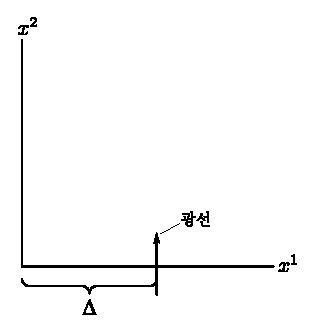
\includegraphics[width=6cm]{Delta.eps}\hfill \,

이에 따르면 태양을 스쳐 지나가는 광선은 $1.7^{\prime\prime}$로 굽어지고, 목성을 스쳐 지나가는 광선은 약 $0.02^{\prime\prime}$로 굽어진다.

중력장을 더 높은 차수의 근사까지 계산하면, 그리고 마찬가지로 상대적으로 극히 작은 질량을 가진 질점의 궤도 운동을 이에 상응하는 정밀도로 계산하면, 행성 운동의 케플러-뉴턴 법칙으로부터 다음과 같은 종류의 편차가 일어남을 발견한다. 즉 타원 궤도가 운동의 방향으로 느리게 돌고, 그 정도는 1 회전당
\begin{equation} \label{eq-75}
	\epsilon=24\pi^3\frac{a^2}{T^2 c^2 \left(1-e^2\right)}
\end{equation}
이다.
이 공식에서 $a$는 장반경의 길이, $c$는 통상적인 척도로 측정한 광속, $e$는 이심률, $T$는 초 단위로 나타낸 주기이다.\footnote{본주: 계산 과정은 원래의 논문 A. Einstein, \emph{Sitzungsberichte der K\"oniglich Preussischen Akademie der Wissenschaften}. 1915, II. pp. 831-839 를 참조함.}

수성에 대한 계산에 따르면 1세기당 $43^{\prime\prime}$의 궤도 회전이 생기며, 이는 르베리에(Leverrier)의 천문학적 관측과 정확히 일치한다. 천문학자들은 이 행성의 근일점의 운동에서, 다른 행성들의 섭동을 고려한 다음, 설명되지 않는 여분으로서 이 값을 발견하였다.  
\end{document}
